%from chapin2013:  An individual bolometer acts as a thermal absorber which are linked directly to transition edge sensors.  When the sensors detect detect thermal variations they will produce changing currents which result in changing magnetic fields.  The magnetic fields are detected by super conduction quantum interference devices (SQUIDs) prior to the output currents being digitized.  Between the initial SQUID amplification and digitization of the current, the data is resampled from 12KHz to 200Hz.  A chain of ``dark SQUIDs'' is used to detect any non-thermal noise that can arise from the amplification of the signal.  //all unnecessary....
\chapter{Observations and Data Preparation}\label{observations}

\section{SCUBA-2} \\
The Submillimetre Common-User Bolometer Array 2 (SCUBA-2) was designed to decrease the observing time of the sub-millimeter sky relative to its predecessor SCUBA \citep{holland2013}.  This would benefit the community by allowing for rapid data acquisition in the submillimeter regime of the electromagnetic spectrum, at the 450$\mu$m and 850$\mu$m bands in particular.  Prior to SCUBA-2, other bolometer cameras such as LABOCA, BOLOCAM and SHARC-II were limited to less than 100 pixels, while the new SCUBA-2 has been able to incorporate over 10,000 pixels in its design and effectively reduce the required observing time \citep{chapin2013}.  Increasing the number of pixels by a factor of 100 was possible by the advent of new technology such as high precision micromachining, superconducting transition edge sensors, and superconducting quantum interference device amplifiers (SQUIDs) \citep{holland2013}.

The observations of NGC3627 were taken from the Nearby Galaxies Legacy Survey's (NGLS) initial science images using SCUBA-2 from December 29, 2011  to January 21, 2012, and consist of 24 18$\arcmin$ by 18$\arcmin$ scans taken in weather conditions where the optical depth of the water in the atmosphere is no greater than $\tau<$0.13.  The observations were centered at 450$\mu$m and 850$\mu$m emission with a 32$\mu$m and 85$\mu$m bandpass, respectively.  16 of the 24 scans were deemed useable, and whether or not an observation was deemed worthwhile was determined by factors such as the behavior of the image background or whether the image was flagged during observing to be unusable.  The observations of NGC3627 were taken using a DAISY scanning pattern  to help remove any random noise by introducing crossing points.  The scanning speed of the JCMT was 150$\arcsec$/second in order to reduce any drifting effects seen from the instrument or sky \citep{chapin2013}.

\section{Image Creation and Properties}\label{sc2_imgs}

For any imaging process to be successful, the final image needs to have minimal white noise \citep{chapin2013}.  White noise in our bolometer observations arises from thermal variations from the instrumentation and atmosphere during data acquisition and is referred to as ranomn noise during the image creation. The random noise is minimized through scanning methods and during image processing \citep{chapin2013}.  To create the final SCUBA-2 data products, we use the Submillimetre User Reduction Facility (SMURF) procedure MAKEMAP.  This procedure reduces the noise of the observations while maintaining the source's emission by incorporating a combination reduction techinques, one of which principal component analysis which will remove any correlated signal and is useful in detecting point sources \citep{chapin2013}.  The second method is a maximum likelihood analysis that will invert the time series of the data then apply a variety of weights to minimize the variance in the inverted time series \citep{janssen1992,chapin2013}.  Both of these methods have proven useful in reducing bolometer data on their own, but due to the size of raw SCUBA-2 data, either method on its own would result in extreme run times or the process becoming resource intensive \citep{chapin2013}.


MAKEMAP breaks down the image creation into several steps performed in iteration in order to successfully reduce any background noise \citep{chapin2013}.  The raw data is modeled by 

\begin{equation}\label{eq:sc2_raw}
  b_i(t) = f \left[ e_i(t)*a_i(t) + g_i*n_c(t)+n_f(t)+n_r(t)\right]
\end{equation}

\noindent such that $b_i(t)$ is the i$^{th}$ bolometer output at time t, $f$ is a scaling factor determined from flat field calibrations, $e_i(t)$ is the extinction at time t for the i$^{th}$ bolometer, $a_i(t)$ is the astronomical signal for i$^{th}$ bolometer at time t,  $g_i*n_c(t)$ is the noise due to the product of the common mode and gain,  $n_f(t)$ is the low-frequency noise, and  $n_r(t)$ is the random noise from the atmosphere or thermal variations in the equipment \citep{chapin2013}.

The steps used in MAKEMAP are designed so they can estimate each noise component of the bolometer signal.  The COM and GAI steps estimate a common mode signal by fitting the average time-series of each bolometer observation.  The next step is EXT, which is used to apply the measured extinction corrections.  Following EXT is FLT to apply high- and low-pass filters to remove any noise features not removed in the COM and GAI filtering.  After the high- and low-pass filters, the AST step is performed.  AST converts the data from a time series to an image and detects sources to be removed from reduction.  The sources removed during this portion of MAKEMAP are intended to be astronomical in nature.  The final step is NOI which determines the noise in the gridded map after each step has been performed and is calculated by isolating the white noise component in equation \ref{eq:sc2_raw}.  A convergence check is then done based on the magnitude of change in each pixel from the previous map and the current version.  If the check fails, the COM, GAI, EXT, and FLT values are recalculated using the AST information obtained from the previous iteration, and the process is repeated until the convergence values are met or the maximum number of iterations has been carried out \citep{chapin2013}.  Creating the data was done locally using scripts to implement MAKEMAP.

In our production of maps, we used the configuration file dimmconfig\_bright \_compact.lis and altered the AST and FLT sections of the image creation by introducing a mask made from Herschel's 250$\mu$m map.  The purpose of the mask was to exclude the target from interfering with the noise minimization as well as to keep any emission from the galaxy from being significantly altered during image production.  The filter size of the high-pass filter was also modified, and an appropriate value was determined to be 175$\arcsec$.  We determined an appropriate high-pass filter size by running a large range of filters from 100$\arcsec$ to 300$\arcsec$ and inspecting the total recovered flux of NGC3627.  A plot of the returned flux values can be seen in Figure \ref{filt_lines}.  A good filter would not show any significant decrease in flux compared to the 350$\mu$m or 500$\mu$m fluxes.  This requirement removes any filters greater than 200$\arcsec$.  Given the flux was nearly constant with filters less than 200$\arcsec$, we chose an appropriate filter size by examining the structure that was returned, in particular how well the spiral arms were recovered for the 850$\mu$m image, and how well the disk was preserved in the 450$\mu$m image.  The spatial effect of the filters can be seen in Figure \ref{450_flt} for 450$\mu$m and Figure \ref{850_flt} for 850$\mu$m.  The maps were returned from MAKEMAP in units of pW with a pixel size of 2$\arcsec$ by 2$\arcsec$ for both the 450$\mu$m and 850$\mu$m.

\begin{figure}
  \centering
  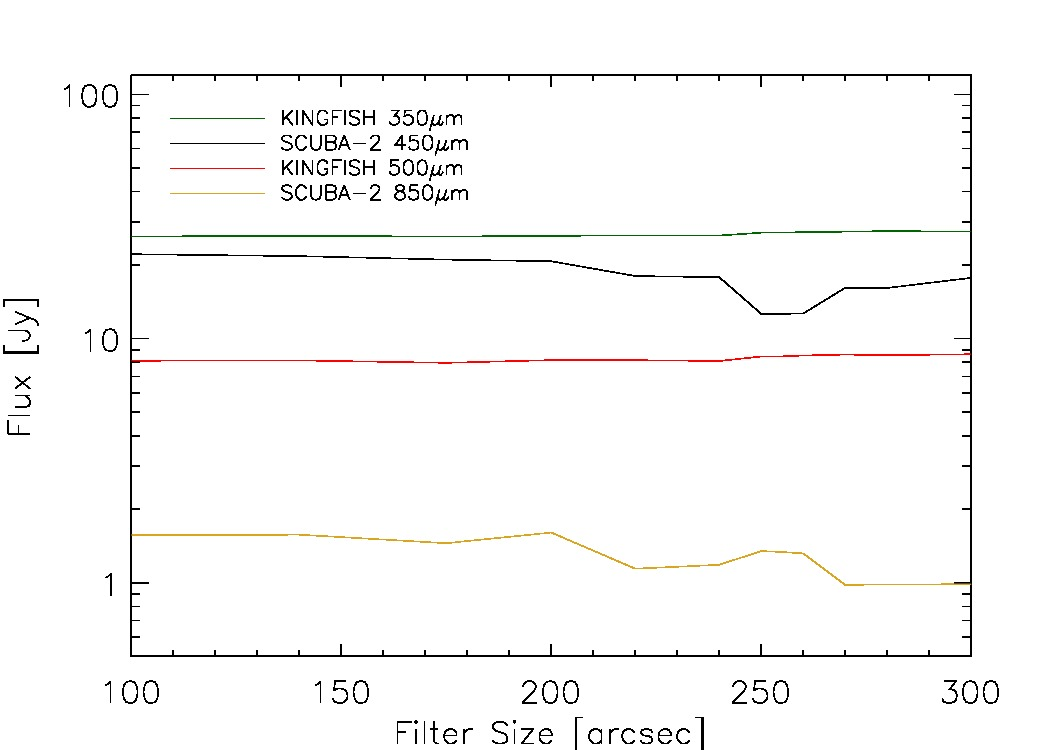
\includegraphics[scale=0.65]{obs_imgs/flux_line.jpeg}
  \caption[Flux Values vs  High-Pass Filter Sizes]{Returned flux values for NGC3627 with varying high-pass filter sizes.  The KINGFISH fluxes have been been processed using the fakesource process, $\S$\ref{fakesource_sec}}
  \label{filt_lines}
\end{figure}

\begin{figure}
  \centering
  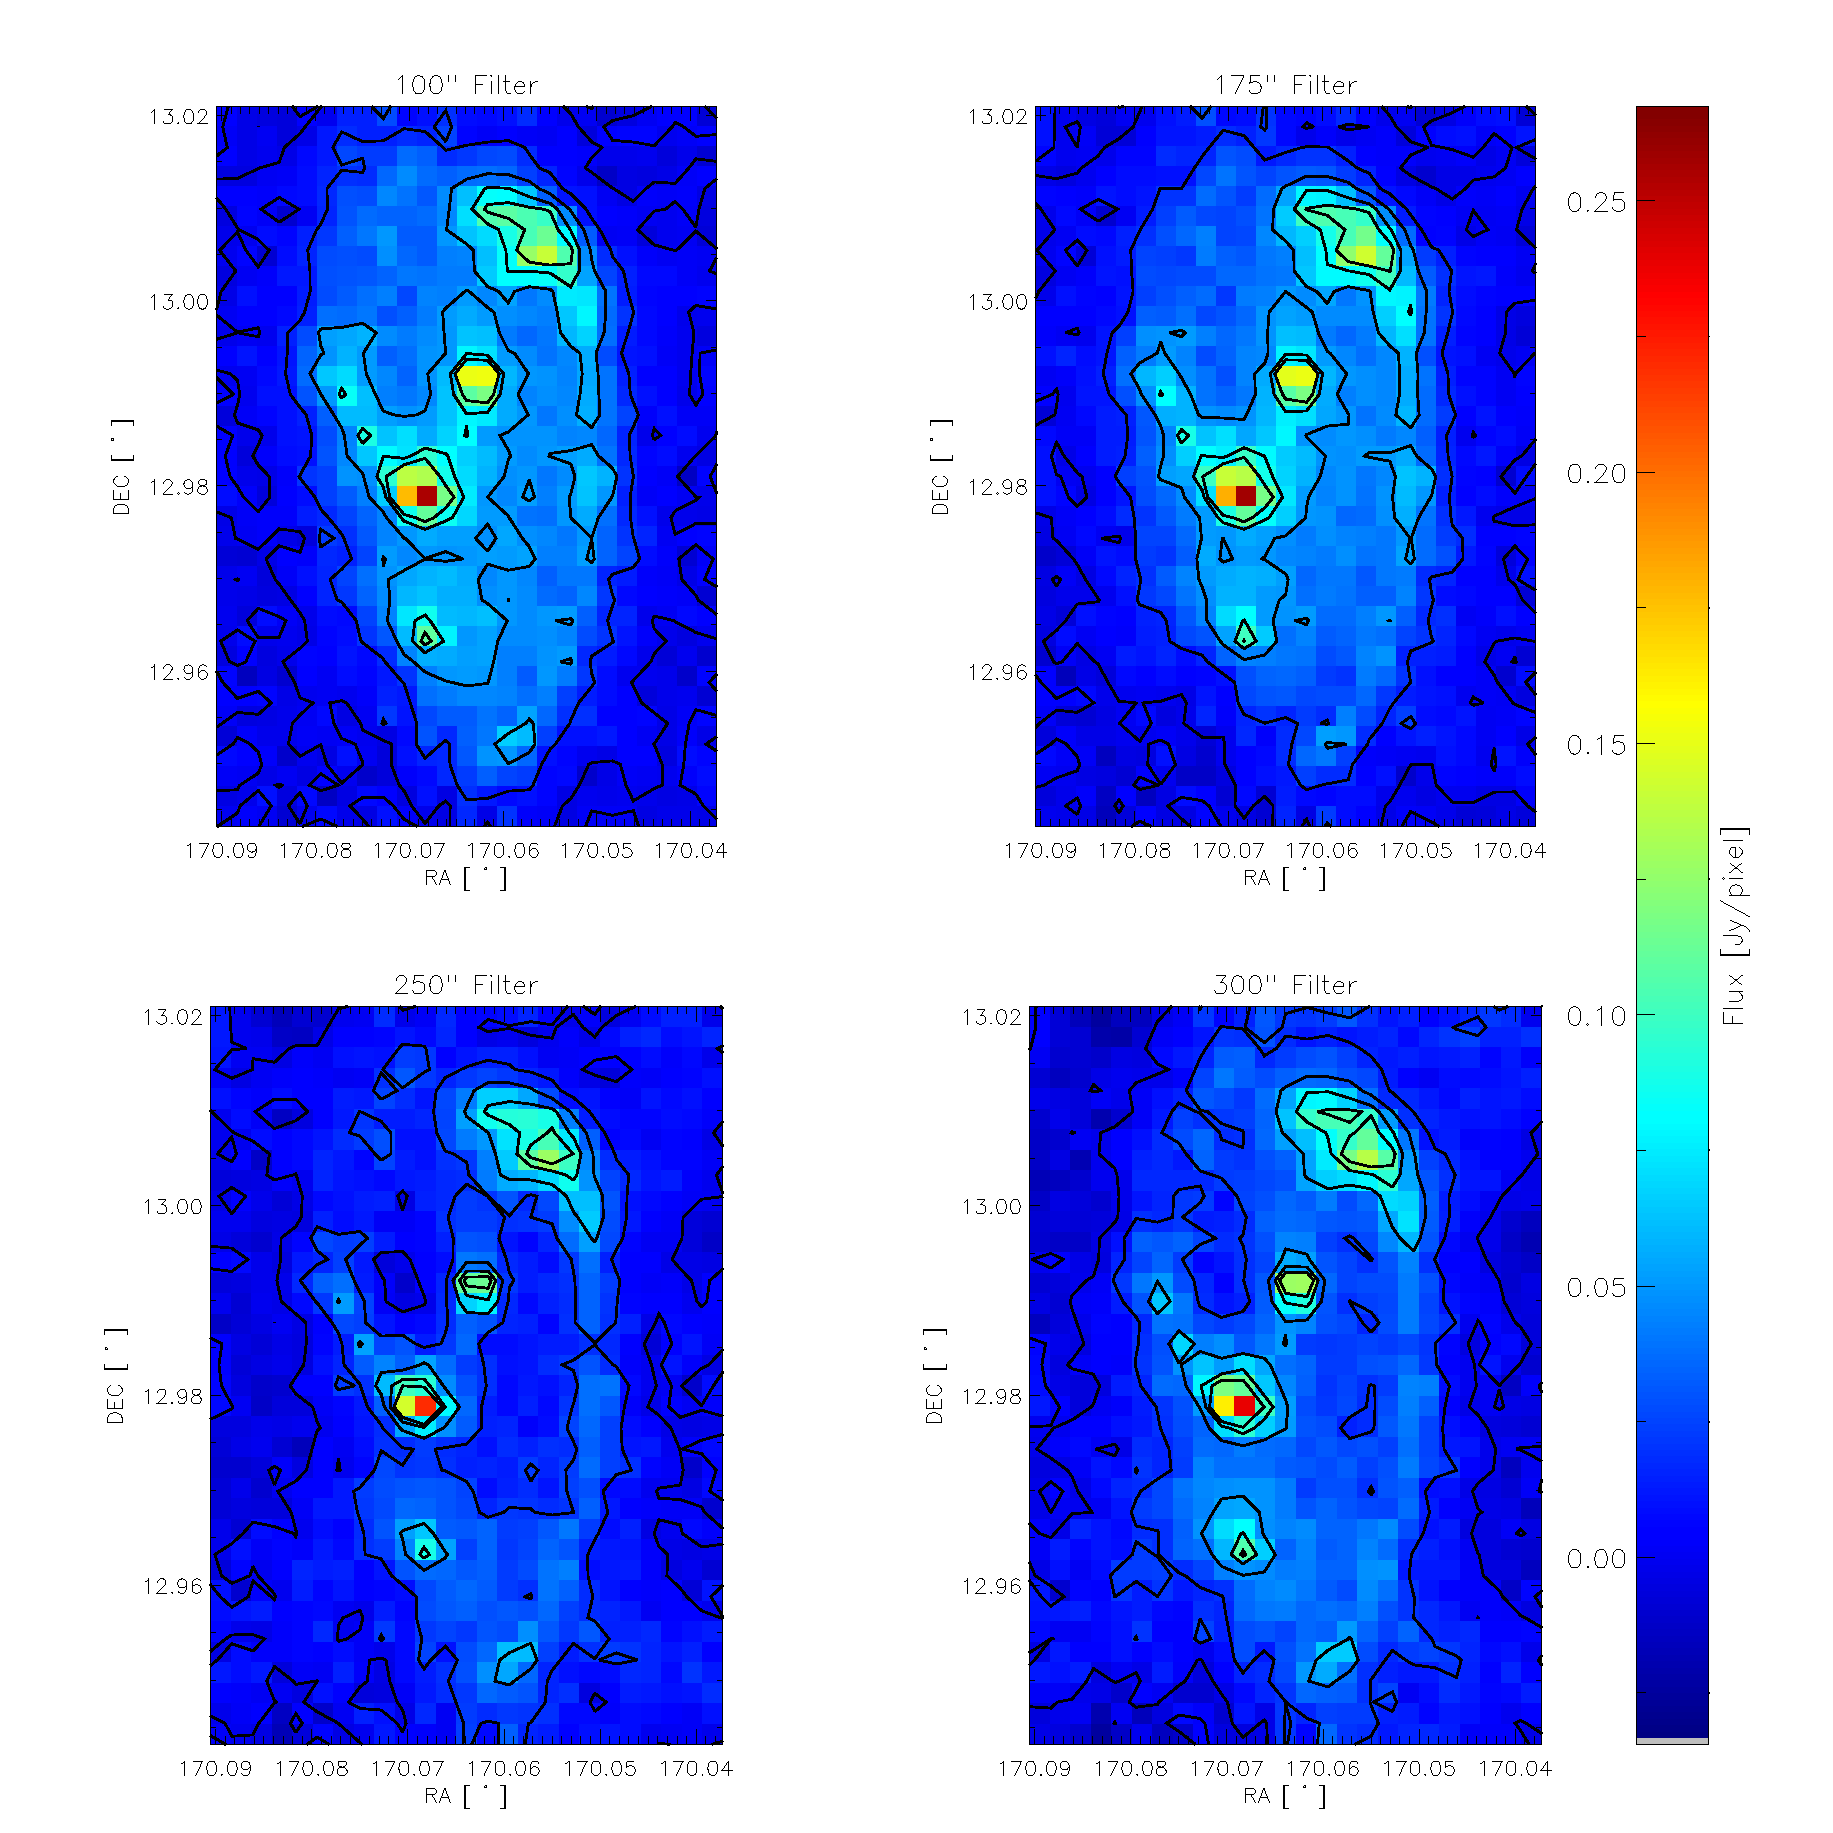
\includegraphics[scale=0.5]{obs_imgs/450_comparison_4.eps}
  \caption[450$\mu$m High-Pass Filter Images]{Four 450$\mu$m maps of NGC3627 using varying high-pass filter sizes.  The contours shown are for 0.0, 0.02, 0.05, 0.08 and 0.1 Jy/pixel for each image with 8$\arcsec$ by 8$\arcsec$ pixels.}
    \label{450_flt}
\end{figure}

\begin{figure}
  \centering
  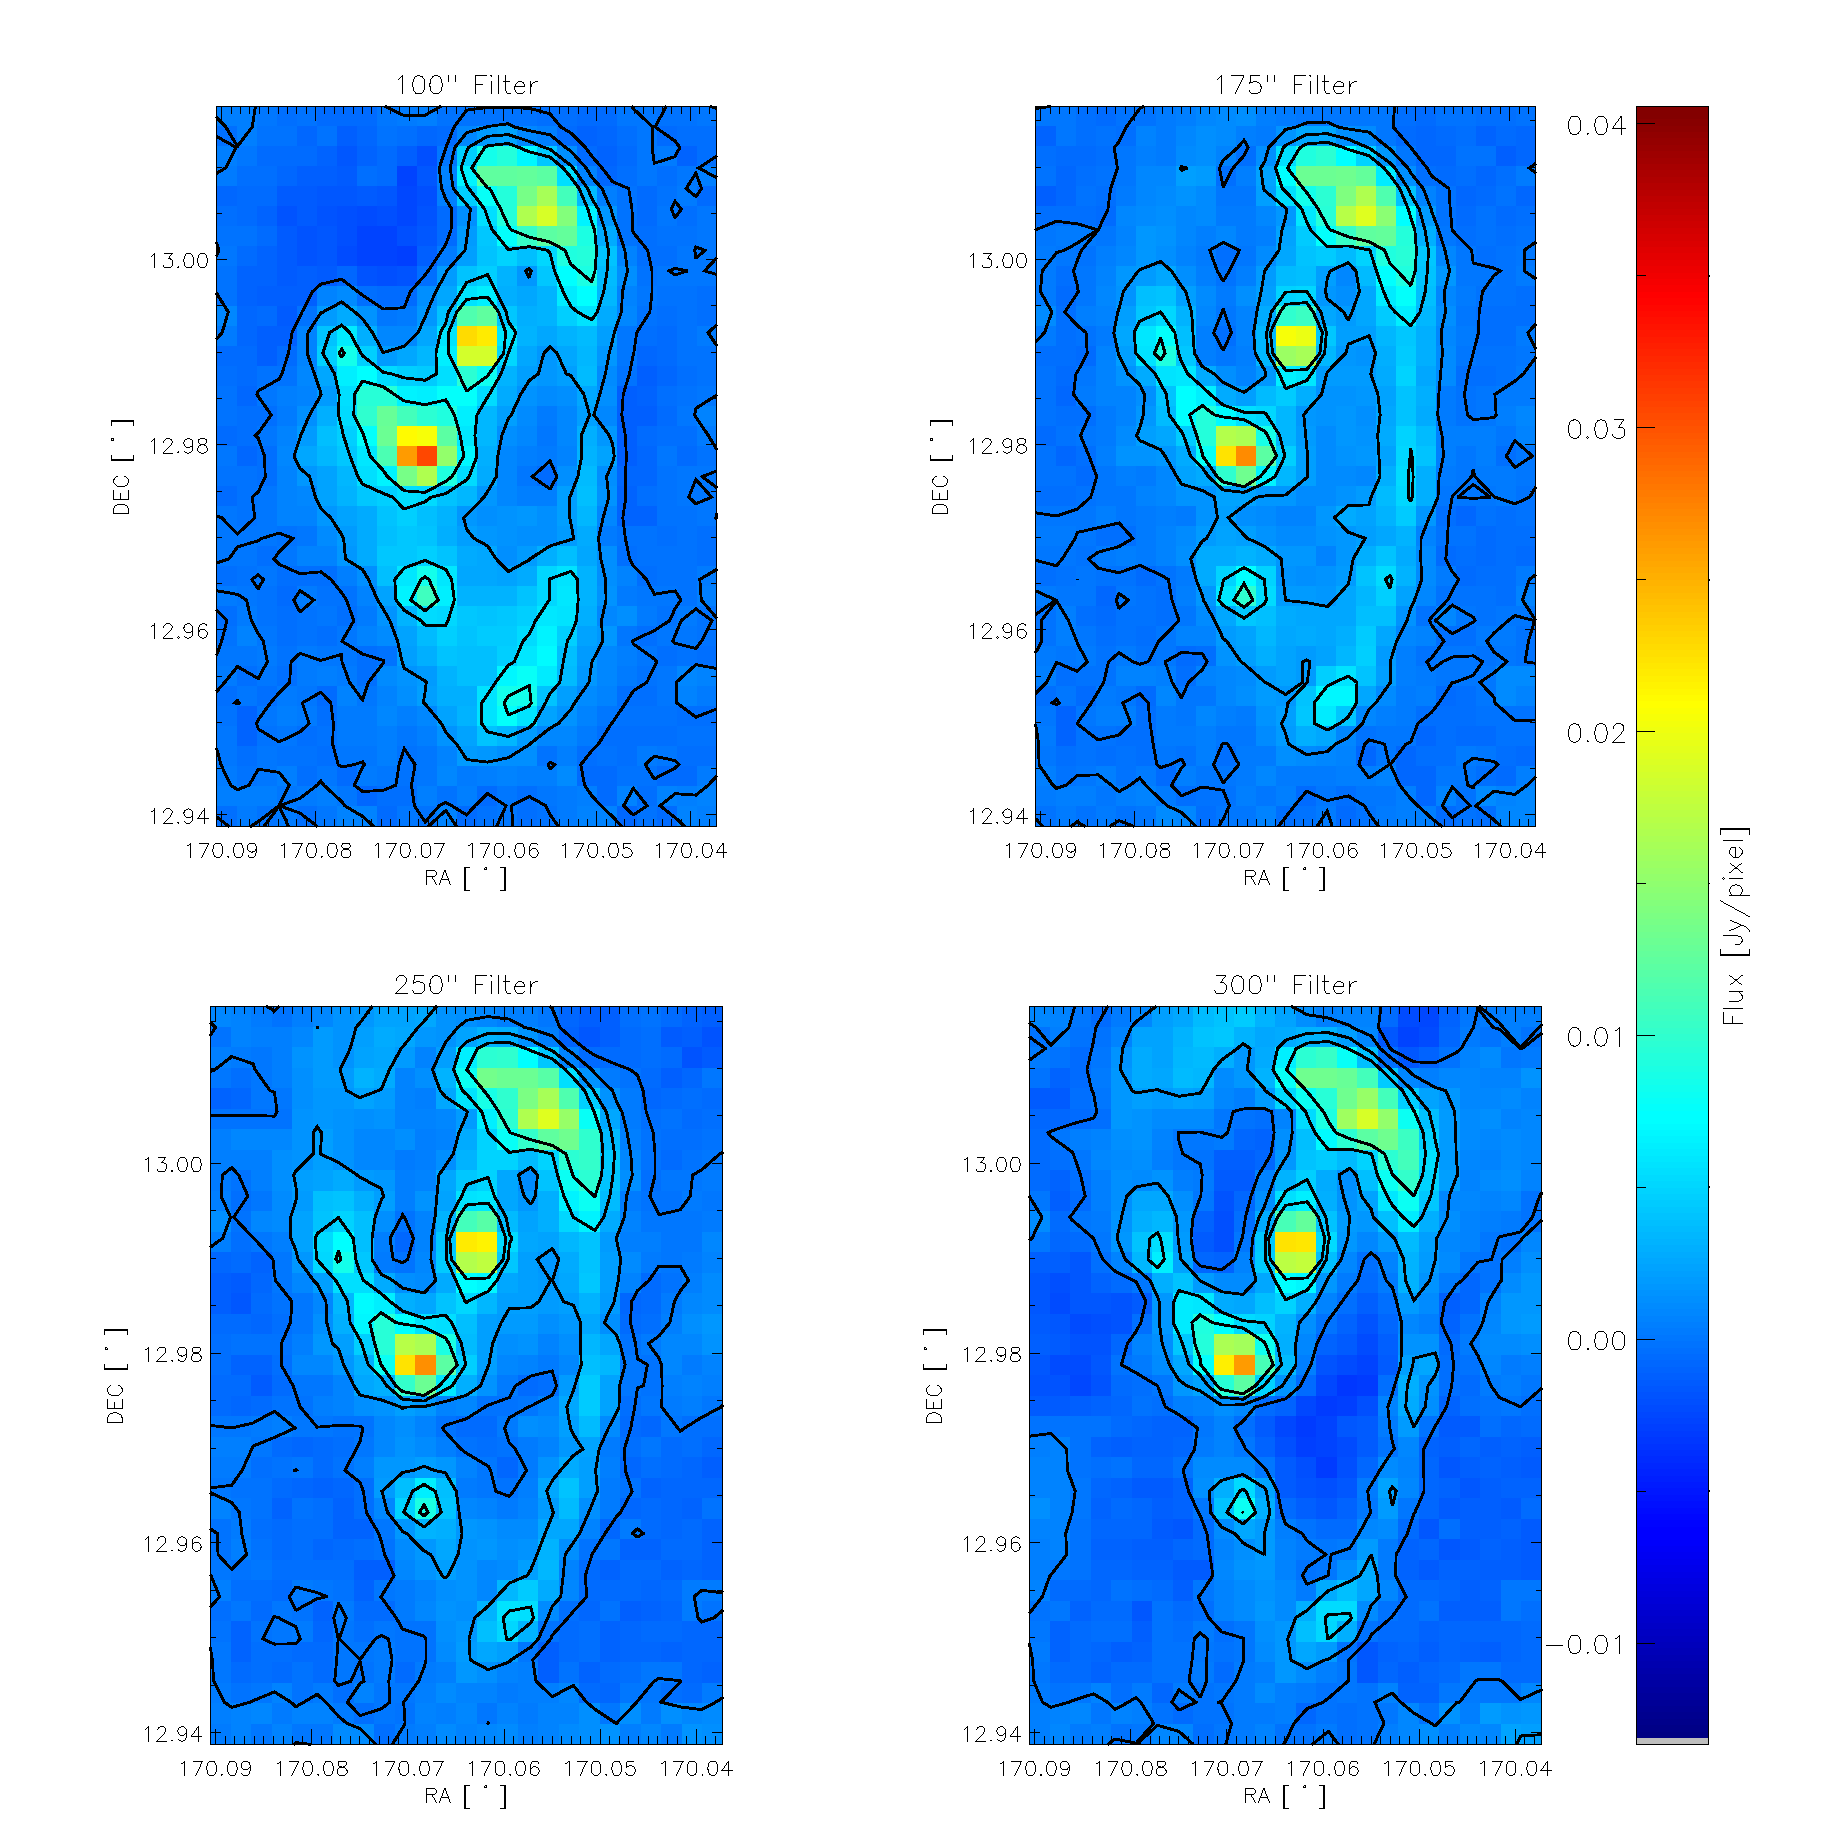
\includegraphics[scale=0.5]{obs_imgs/850_comparison_4.eps}
  \caption[850$\mu$m High-Pass Filter Images]{Four 850$\mu$m maps of NGC3627 using varying high-pass filter sizes.  The contours shown are for 0.0, 0.002, 0.005, and 0.008 Jy/pixel for each image with 8$\arcsec$ by 8$\arcsec$ pixels.}
    \label{850_flt}
\end{figure}

The final 450$\mu$m image was then re-gridded down to a 4$\arcsec$ by 4$\arcsec$ pixel grid, and flux calibration values of 491000 and 4710 \citep{dempsey2013} were applied to convert from pW to mJy/beam and mJy/square arcsecond, respectively.  The 850$\mu$m maps were re-gridded to an 8$\arcsec$ by 8$\arcsec$ pixel size and used flux calibration values of 537000 and 2340 for mJy/beam and mJy/square arcsecond \citep{dempsey2013}.  The 4$\arcsec$ and 8$\arcsec$ pixels correspond to a 180pc and 360pc size scale for our target, NGC3627.  To simplify the analysis, the images are also converted to Jy/pixel.  The 450$\mu$m and 850$\mu$m images are shown in Figures \ref{fig_450} and \ref{fig_850}.  The calibration values used are the default flux calibration factors that are determined from our calibrator source, Uranus, in  \citep{dempsey2013}.  The overall noise in the final image can be seen in Table \ref{tab_obs_scuba2}.

\begin{figure}
  \centering
  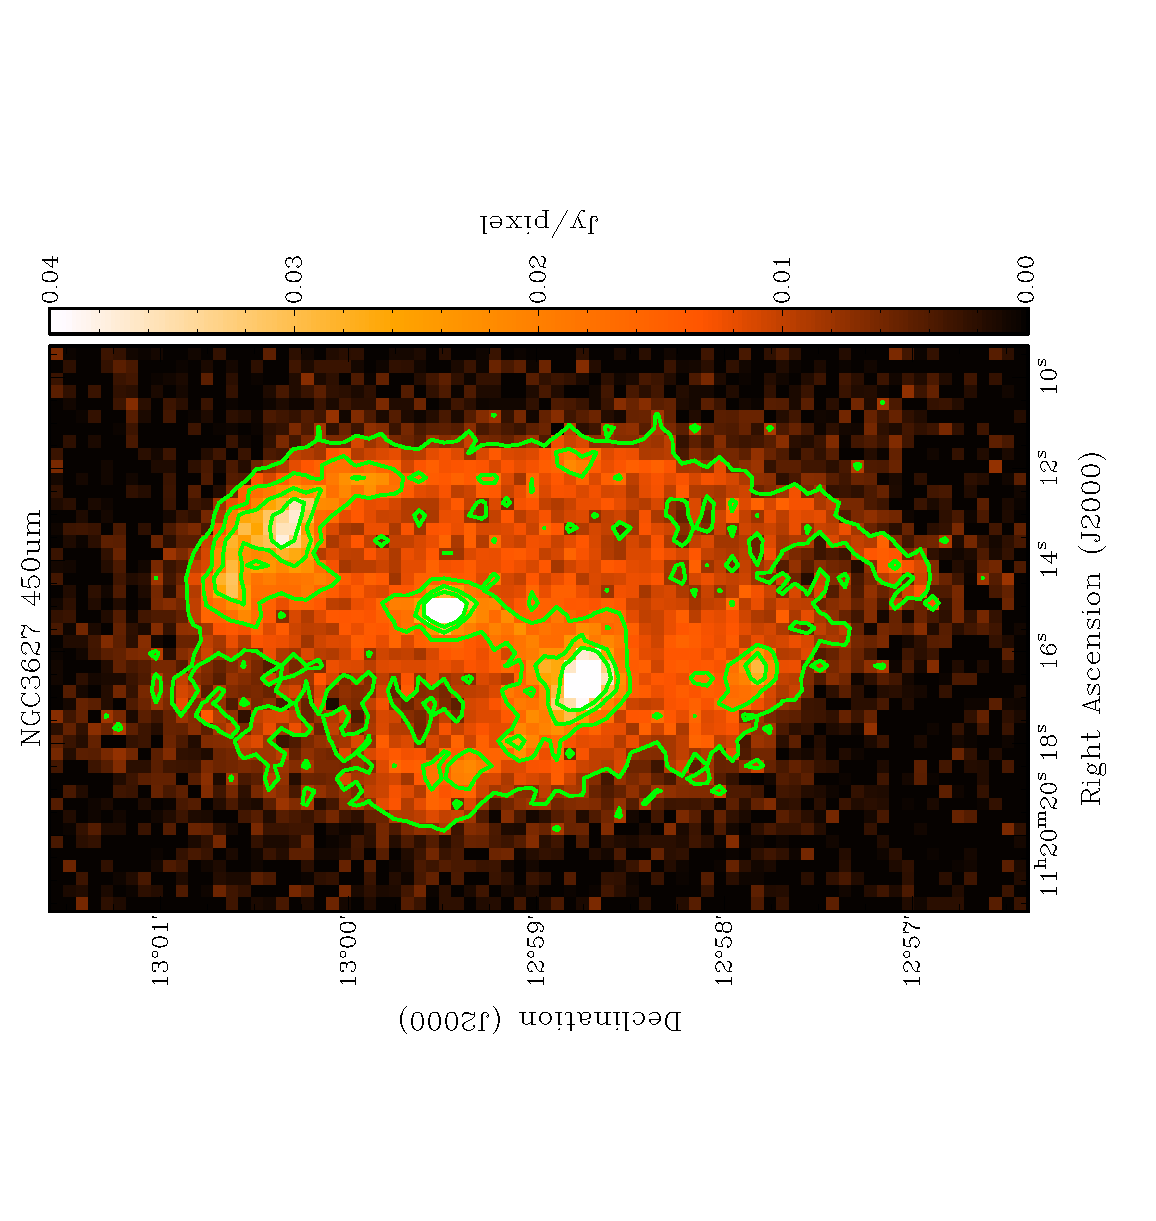
\includegraphics[width=1.\textwidth,angle=270]{obs_imgs/450_um.eps}
  \caption[NGC3627 450$\mu$m Observations]{450$\mu$m observation produced at the end of the image production with 20\%, 40\%, 60\%, and 80\% contours with 4$\arcsec$ by 4$\arcsec$ pixels.}
    \label{fig_450}
\end{figure}

\begin{figure}
  \centering
  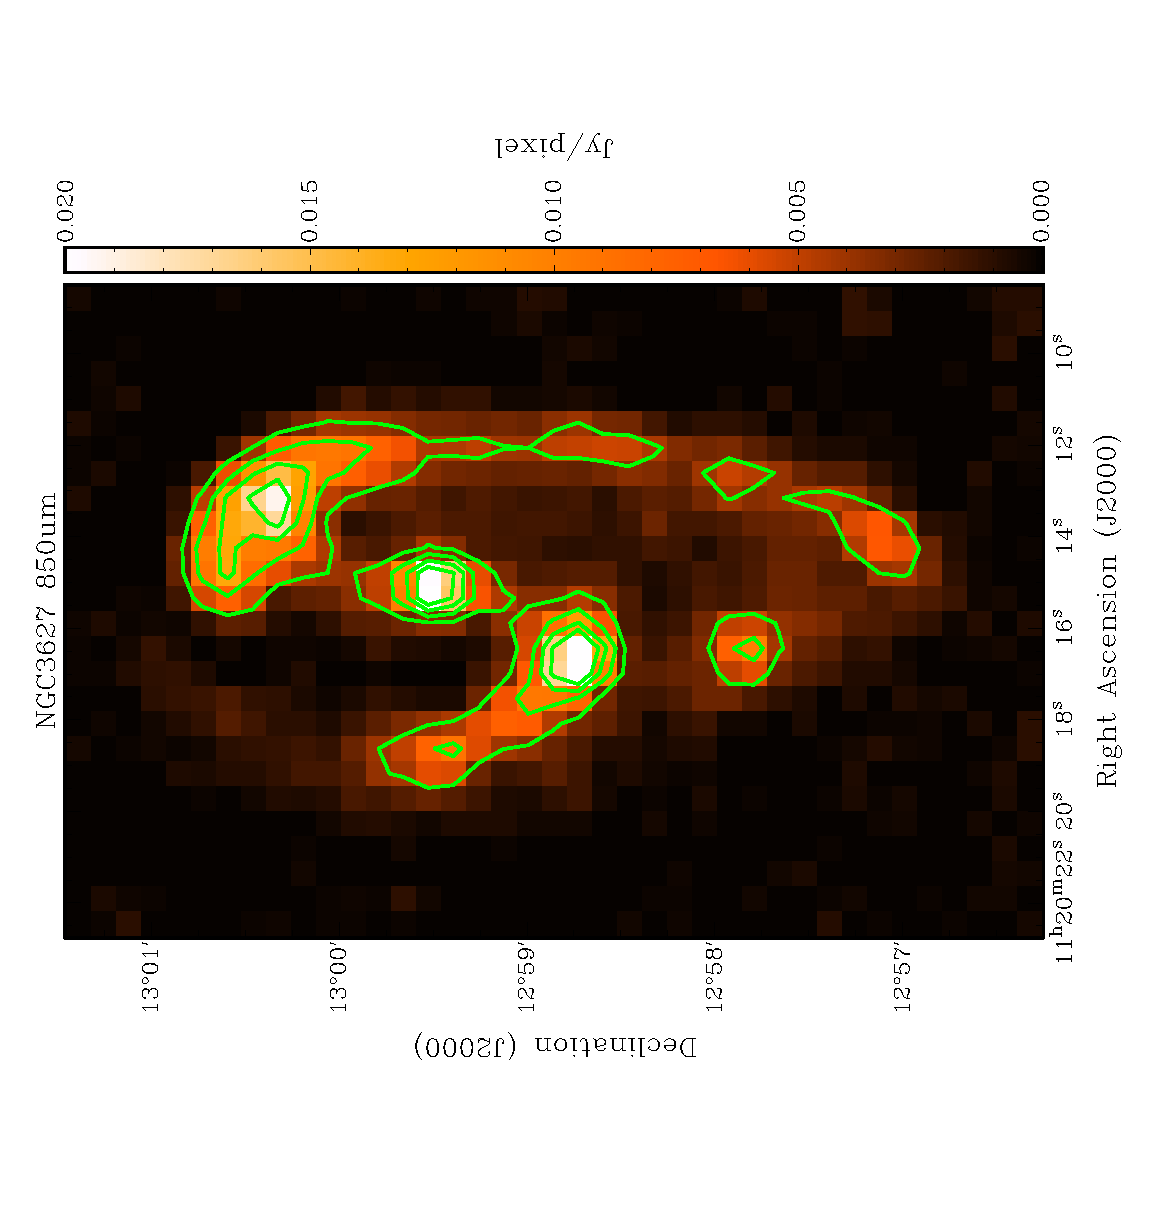
\includegraphics[width=1.\textwidth,angle=270]{obs_imgs/850_um.eps}
  \caption[NGC3627 850$\mu$m Observations]{850$\mu$m observation produced at the end of the image production with 20\%, 40\%, 60\%, and 80\% contours with 8$\arcsec$ by 8$\arcsec$ pixels.}
    \label{fig_850}
\end{figure}

\begin{deluxetable}{cccccc}
  \tabletypesize{\footnotesize}
  \tablecolumns{6}
  \tablewidth{0pt}
  \tablecaption{Properties of NGC3627 SCUBA-2 Observations\label{tab_obs_scuba2}}
  \tablehead{\colhead{Observation} & \multicolumn{4}{c}{Beam Properties} & \colhead{RMS} \\
& Main Beam Amplitude & Main Beam FWHM & Error Beam Amplitude & Error Beam FWHM & \it{[mJy / Pixel]}}
  \startdata
    450$\mu$m & 0.854 $\pm$ 0.002 & 7.48$\arcsec$ $\pm$ 0.03$\arcsec$ & 0.146 $\pm$ 0.003 & 23.1$\arcsec$ $\pm$ 0.2$\arcsec$ & 3.42  \\
    850$\mu$m & 0.9624 $\pm$ 0.0002 & 12.8$\arcsec$ $\pm$ 0.004$\arcsec$ & 0.0376 $\pm$ 0.0002 & 44.5$\arcsec$ $\pm$ 0.09$\arcsec$ &  0.476 \\
   \enddata
\end{deluxetable}

\subsection{Beam Shape of the 450$\mu$m and 850$\mu$m Data} \\
Calibration images of Uranus were used to determine the shape of the beam for the 450$\mu$m and 850$\mu$m observations.  The beam shape of both the 450$\mu$m and 850$\mu$m maps deviates from a single gaussian due to the second maximum of the airy diffraction pattern in the response function of the telescope and minor imperfections in the mirror of the JCMT due to boundaries of the panels \citep{dempsey2013}.  This abnormality is best represented by a sum of two gaussians whose amplitudes sum to unity \citep{dempsey2013}.  The average beam resolutions for the 450$\mu$m and 850$\mu$m data are reported in Table \ref{tab_obs_scuba2} and are within an acceptable difference from the values found in \cite{dempsey2013} since we used only the nights our data was taken compared to the work done by \cite{dempsey2013} that used observations taken over a year.  The calibration images, fitted beams, and the residual of the fits can be seen in Figure \ref{fig_calib}.  The residuals seen in here are due to asymmetries in the Uranus PSF.  The contribution of the error beam in the 850$\mu$m emission is negligible, and allows the beam to be approximated by a single gaussian.  However, the contribution of the error beam in the 450$\mu$m images was large enough to require special treatment in order to properly match the beams for analysis.

\begin{figure}
  \centering
  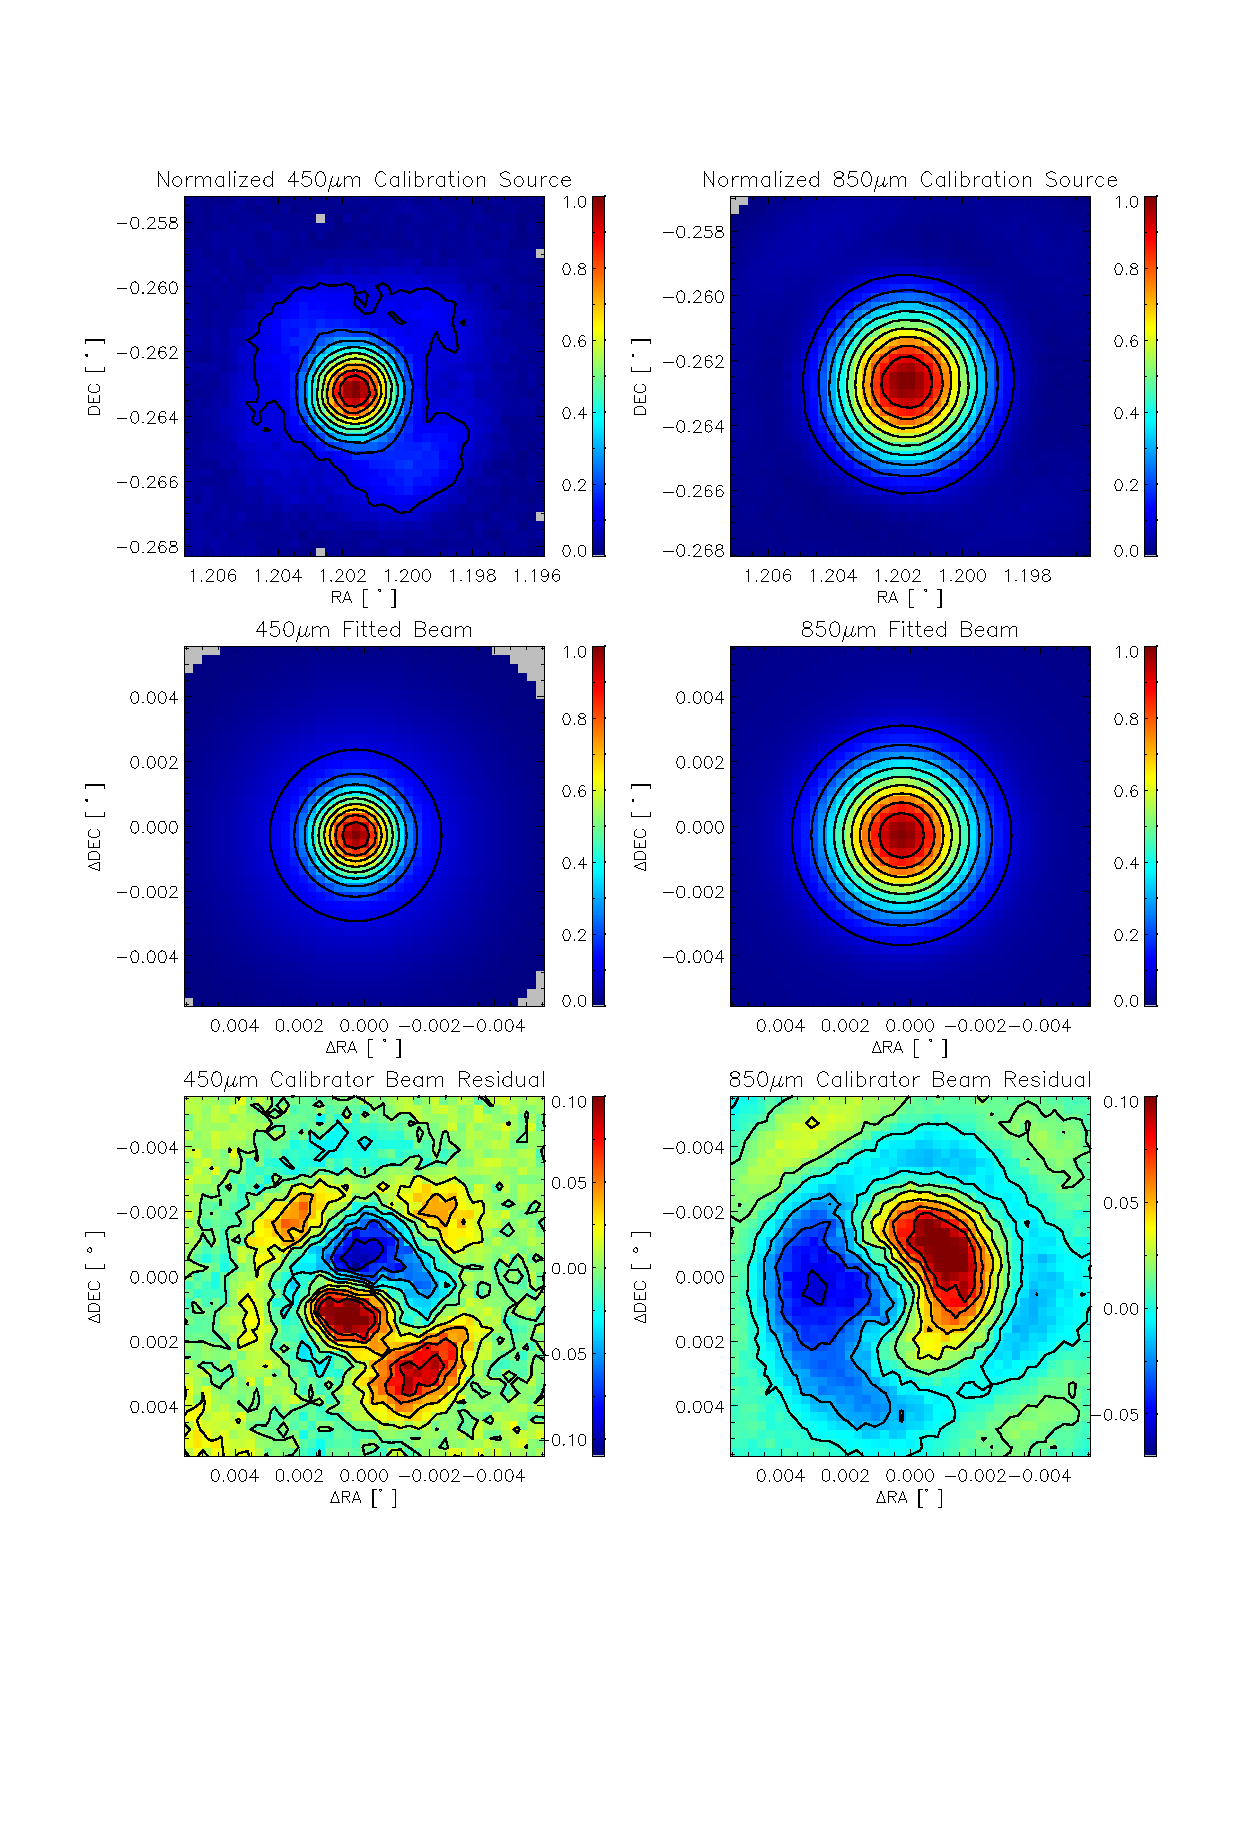
\includegraphics[width=1.\textwidth, trim={0 5cm 0 0}]{obs_imgs/calib_beams.eps}
  \caption[SCUBA-2 Calibration and Beams]{The top row shows the Uranus images taken on January, 8th 2012 for 450$\mu$m on the left and 850$\mu$m on the right.  The middle row shows the fitted beams for 450$\mu$m on the right and 850$\mu$m on the left using the double gaussian beam shape. The bottom row shows the difference between the original image and the fitted beam.  The contours in the image are from 10\% to 90\% in intervals of 10\%.}
    \label{fig_calib}
\end{figure}

\section{Ancillary Data}\label{ancillary}

The scientific goals of this thesis require data outside the capabilities of SCUBA-2.  For instance, accurately determining the dust mass involves fitting the spectral energy distribution (SED) for NGC3627.  To successfully fit an SED, we need shorter wavelength data to fully probe the cold component of this galaxy. We used data ranging from 100$\mu$m to 500$\mu$m from the KINGFISH survey \citep{kennicutt2011} to gain a large enough wavelength range for fitting the cold component.  Secondly, the bandpass of the 850$\mu$m filter contains the CO J=3-2 line.  In order to get a valid measurement of the dust mass, this contribution had to be removed.  We used emission data from the NGLS from the HARP instrument on the JCMT \citep{wilson2012} to remove this contamination.  When a dust mass was obtained, we used CO J=1-0 from the Nobeyama 45-m telescope \citep{kuno2007}, CO J=2-1 from HERACLES \citep{leroy2009}, and $HI$ observations from THINGS \citep{walter2008} to determine a reasonable molecular hydrogen mass to calculate a dust-to-gas ratio.  In the next sections we give some details for these ancillary data sets.

\subsection{Key Insights on Nearby Galaxies: a Far-Infrared Survey with Herschel (KINGFISH)}

The Key Insights on Nearby Galaxies: a Far-Infrared Survey with Herschel (KINGSFISH) was designed to be a follow up to the Spitzer Infrared Nearby Galaxies Survey (SINGS) \citep{kennicutt2003} with observations of the warm and cold component of dust emission using the increased resolution from Herschel \citep{kennicutt2011}.  The main science goals of the KINGFISH survey were to better understand the star formation processes that were shielded by dust, to make resolved studies of heating and cooling of the interstellar medium (ISM), and to build an inventory of how cold dust emission relates to other dust components in the ISM \citep{kennicutt2011}.  The survey consists of 61 nearby galaxies (d$<$30Mpc) that cover a range of environments.  Each target was observed at 70$\mu$m, 100$\mu$m, 160$\mu$m, 250$\mu$m, 350$\mu$m, and 500$\mu$m.  Our analyis focuses on fitting the cold component of NGC3627's SED, so we omitted the 70$\mu$m emission from the fitting, and processed the data through MAKEMAP as described below in $\S$ \ref{data_agree}.  The rms and beam size after the large scale structure has been removed can be seen in Table \ref{tab_obs_kfish} given for 8$\arcsec$ by 8$\arcsec$ pixels, while the preconvolved maps are shown in Figures \ref{fig_100} to \ref{fig_500}.

\begin{figure}
  \centering
  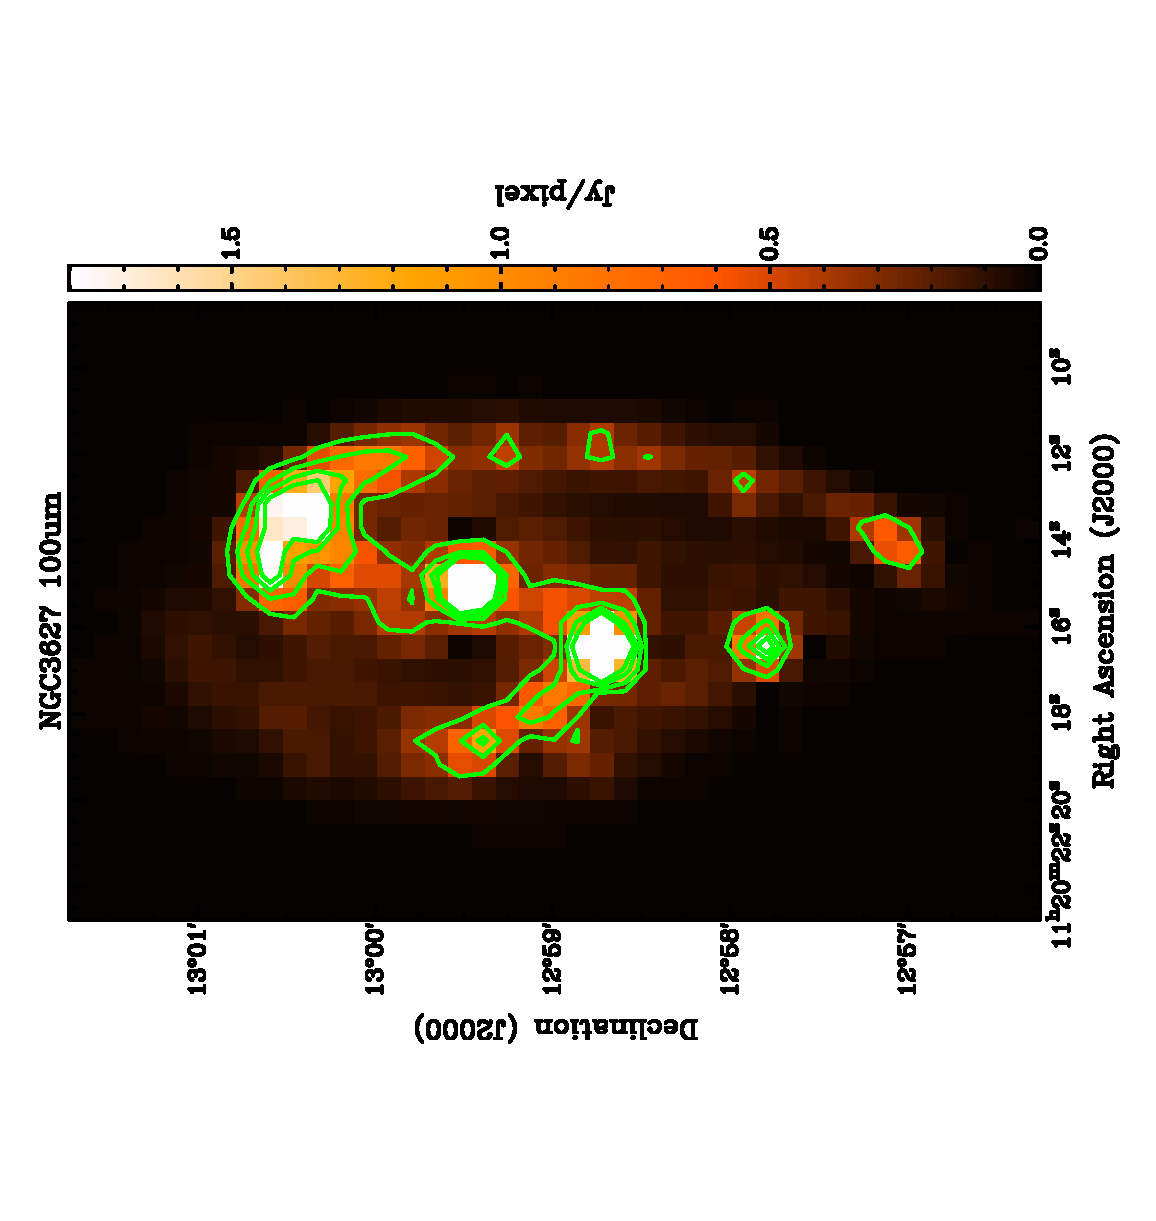
\includegraphics[width=1.\textwidth,angle=270]{obs_imgs/100_rem.eps}
  \caption[NGC3627 100$\mu$m Observations]{Image after the MAKEMAP filtering of 100$\mu$m observations with 20\%, 40\%, 60\%, and 80\% contours.}
  \label{fig_100}
\end{figure}

\begin{figure}
  \centering
  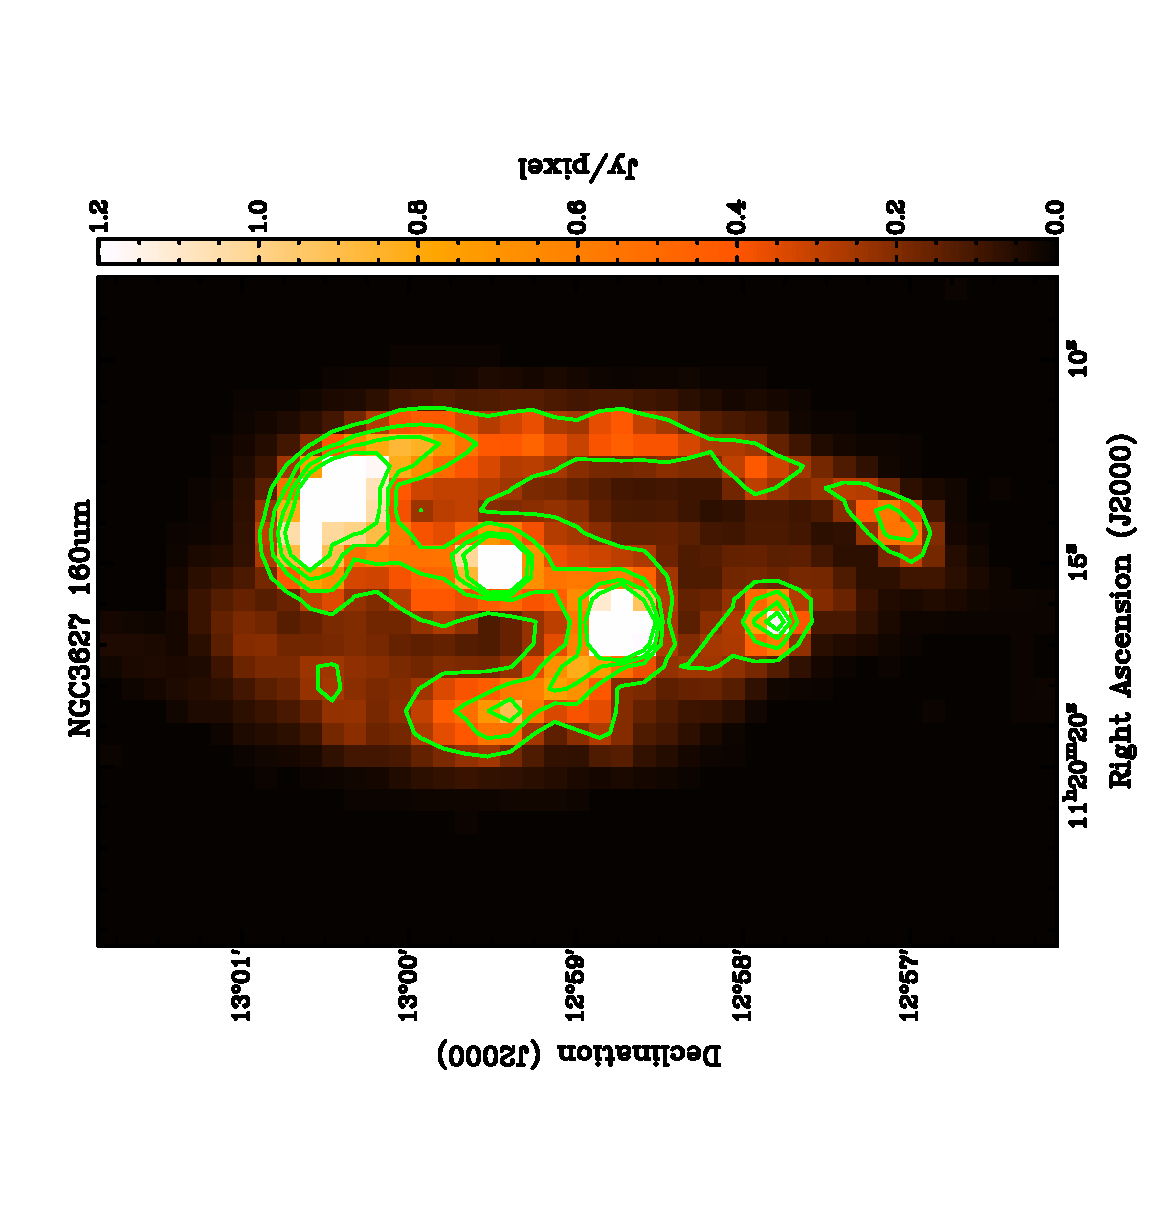
\includegraphics[width=1.\textwidth,angle=270]{obs_imgs/160_rem.eps}
  \caption[NGC3627 160$\mu$m Observations]{Image after the MAKEMAP filtering of 160$\mu$m observations with 20\%, 40\%, 60\%, and 80\% contours.}
  \label{fig_160}
\end{figure}

\begin{figure}
  \centering
  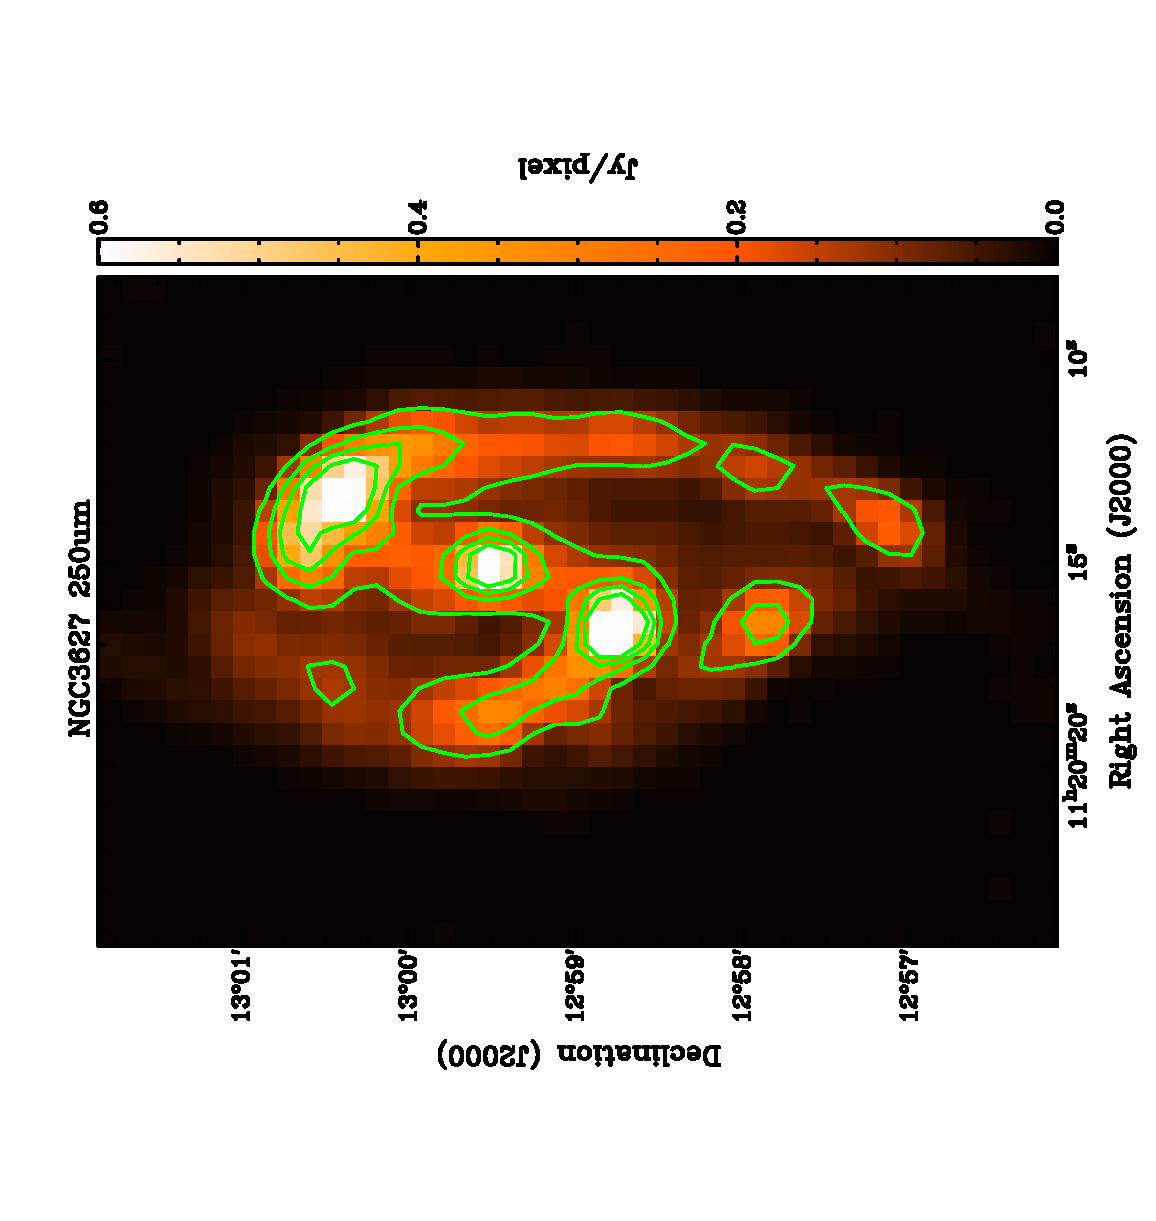
\includegraphics[width=1.\textwidth,angle=270]{obs_imgs/250_rem.eps}
  \caption[NGC3627 250$\mu$m Observations]{Image after the MAKEMAP filtering of 250$\mu$m observations with 20\%, 40\%, 60\%, and 80\% contours.}
  \label{fig_250}
\end{figure}

\begin{figure}
  \centering
  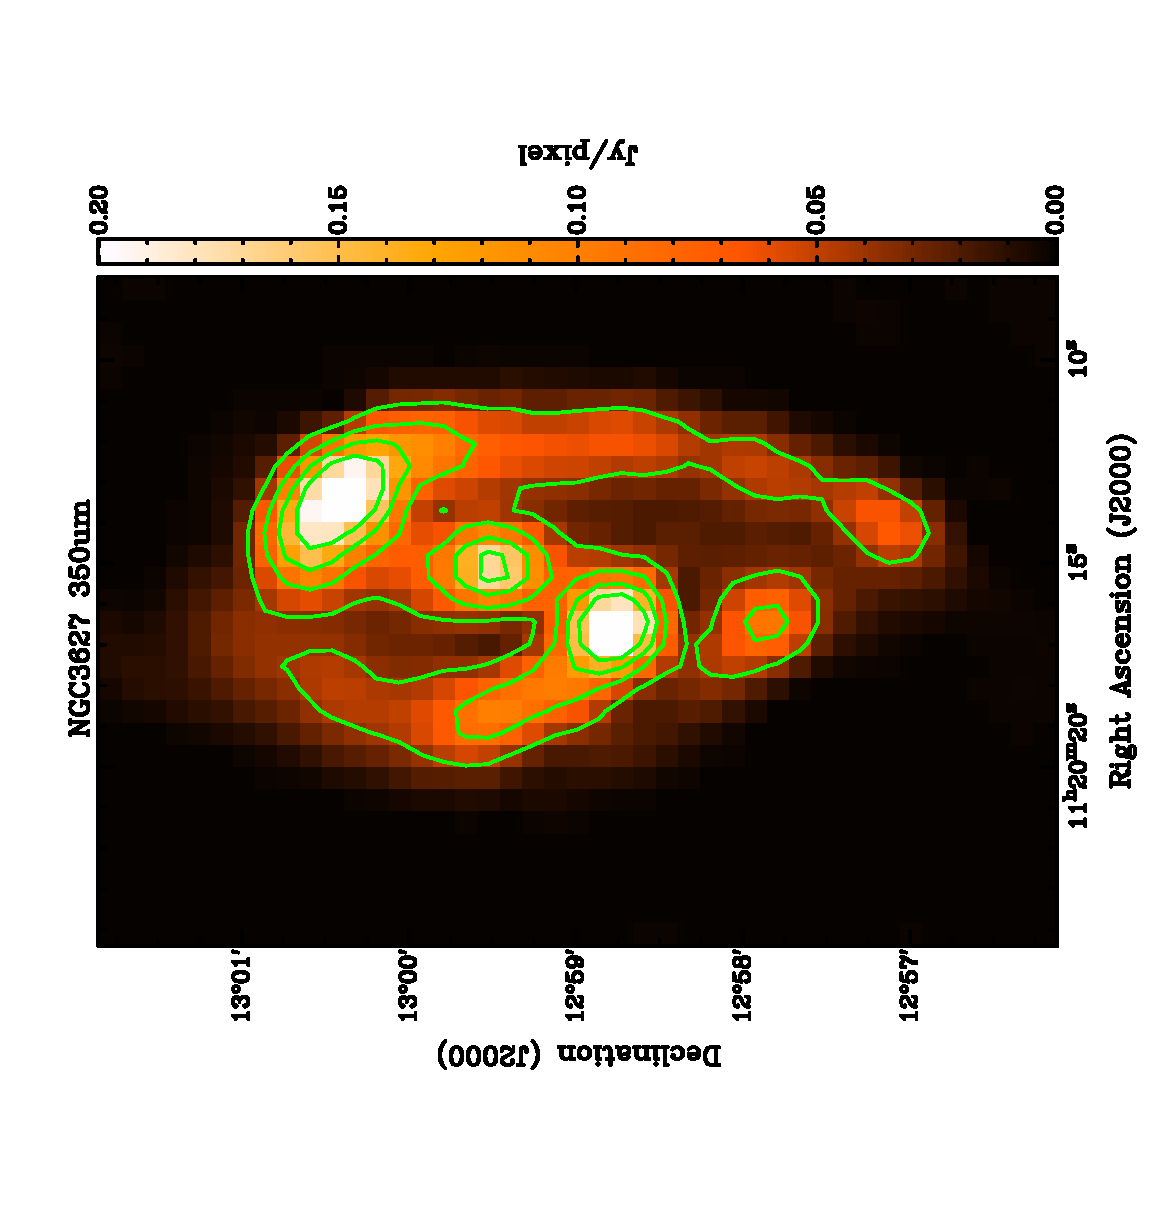
\includegraphics[width=1.\textwidth,angle=270]{obs_imgs/350_rem.eps}
  \caption[NGC3627 350$\mu$m Observations]{Image after the MAKEMAP filtering of the 350$\mu$m observations with 20\%, 40\%, 60\%, and 80\% contours.}
  \label{fig_350}
\end{figure}

\begin{figure}
  \centering
  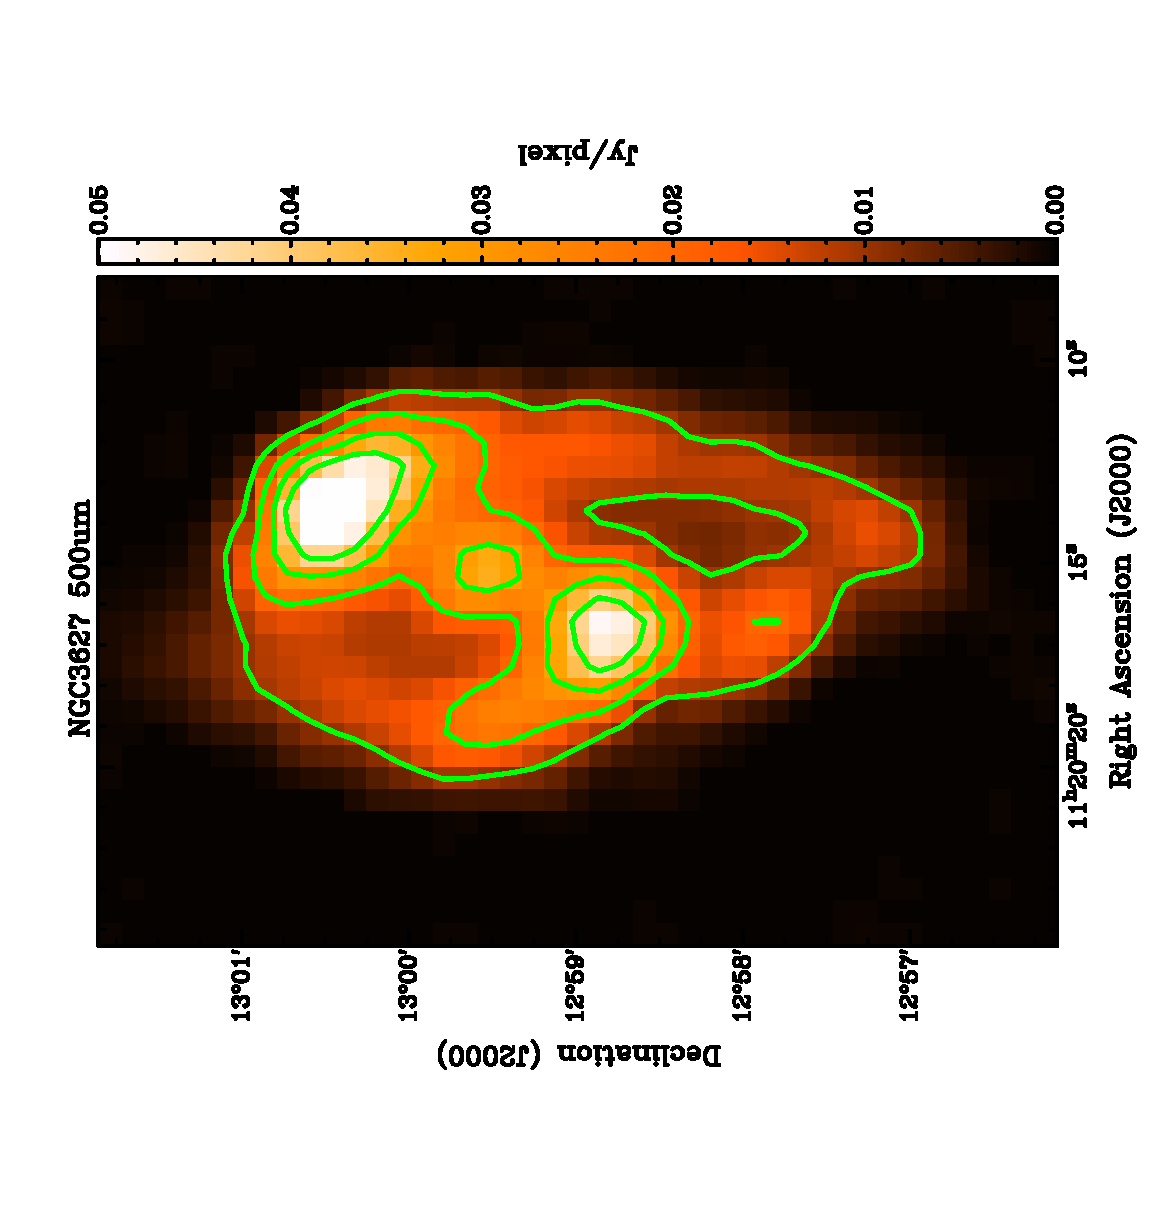
\includegraphics[width=1.\textwidth,angle=270]{obs_imgs/500_rem.eps}
  \caption[NGC3627 500$\mu$m Observations]{Image after the MAKEMAP filtering of the 500$\mu$m observations with 20\%, 40\%, 60\%, and 80\% contours.}
  \label{fig_500}
\end{figure}

\begin{deluxetable}{cccc}
%  \table{\footnotesize}
  \tablecolumns{4}
  \tablewidth{0pt}
  \tablecaption{Properties of NGC3627 KINGFISH Observations\label{tab_obs_kfish}}
  \tablehead{\colhead{Observation} & \colhead{Beam Properties } & \colhead{RMS} & \colhead{Percentage of Emission Removed} \\
 & $\theta_{beam}$ & \it{[mJy/Pixel]}}
  \startdata
    100$\mu$m & 6.8$\arcsec$ & 2.24 & 11\% \\
    160$\mu$m & 11.6$\arcsec$ & 3.95 & 17\% \\
    250$\mu$m & 18.0$\arcsec$ & 2.47 & 20\% \\
    350$\mu$m & 24.9$\arcsec$ & 1.08 & 21\% \\
    500$\mu$m & 36.0$\arcsec$ & 0.387 & 28\% \\
  \enddata
\end{deluxetable}

\subsection{Nearby Galaxies Legacy Survey (NGLS)}

The Nearby Galaxies Legacy Survey is an HI-selected set of 155 galaxies contained with distances between 2 and 25 Mpc observed using the instrumentation on the JCMT \citep{wilson2012}.  The NGLS consists of multiwavelenght data that include the 450$\mu$m and 850$\mu$m data used for this thesis.  As mentioned previously, the bandpass for SCUBA-2's 850$\mu$m emission contains the CO J=3-2 line which is contained in the NGLS data set.  We used the zeroth moment CO J=3-2 maps from the NGLS to determine the percentage of CO J=3-2 emission present in the 850$\mu$m band as well as removing it for an accurate SED analysis.  The rms and resolution of the CO J=3-2 emission are shown in Table \ref{tab_obs_NGLS} for 8$\arcsec$ by 8 $\arcsec$ pixels, and the scan prior to convolution is shown in Figure \ref{fig_co32}.

\begin{figure}
  \centering
  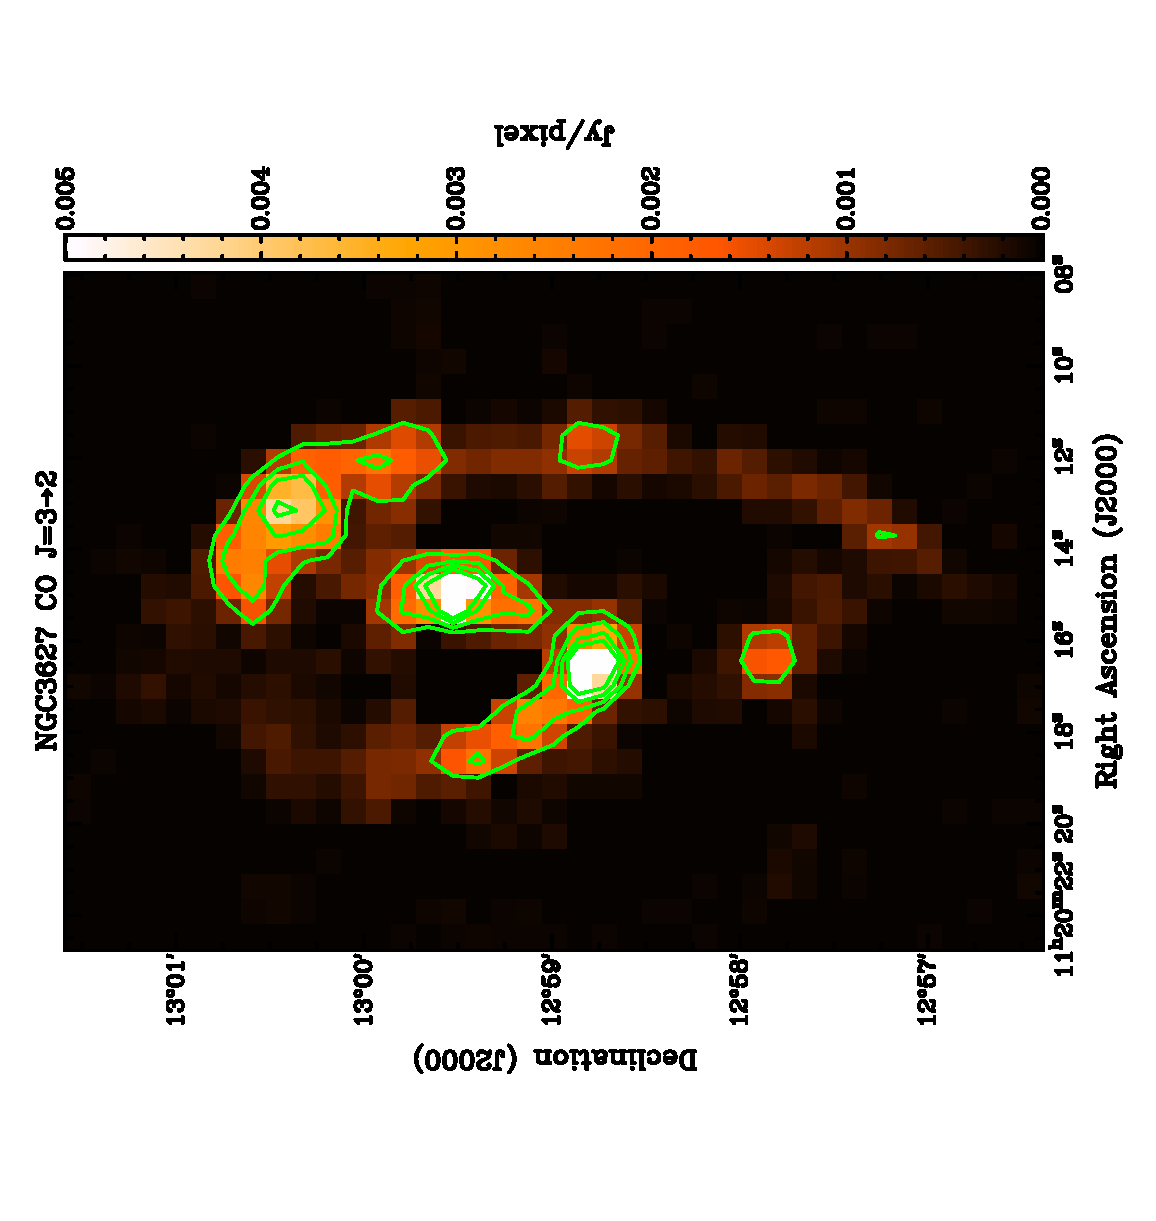
\includegraphics[width=1.\textwidth, angle=270]{obs_imgs/32_rem.eps}
  \caption[NGC3627 CO J=3-2 Observations]{Residual of the MAKEMAP filtering of CO J=3-2 observations used to subtract line contamination from 850$\mu$m SCUBA-2 map with 20\%, 40\%, 60\%, and 80\% contours.}
  \label{fig_co32}
\end{figure}

\begin{deluxetable}{cccc}
  \tablecolumns{4}
  \tablewidth{0pt}
  \tablecaption{Properties of NGC3627 NGLS Observations\label{tab_obs_NGLS}}
  \tablehead{\colhead{Observation} & \colhead{Beam Properties } & \colhead{RMS} & \colhead{Percentage of Emission Removed} \\
 & $\theta_{beam}$ & \it{[mJy/Pixel]}}
  \startdata
    CO J=3-2 & 14.5$\arcsec$ & 1.28e-2& 29.8\% \\
  \enddata
\end{deluxetable}

%insert co32 img

\subsection{Nobeyama 45-m}\label{nob_sec}

Determining a dust-to-gas ratio requires a molecular tracer to estimate the amount of molecular hydrogen present.  The most frequently used tracer is CO J=1-0 due to its abundance in the ISM.  The CO J=1-0 data were obtained from the Nobeyama 45-m CO Atlas of Nearby Spiral Galaxies \citep{kuno2007}.  The Nobeyama 45-m CO Atlas consists of galaxies with morphologies ranging from Sa to Scd, located less than 25Mpc from the Milky Way, inclination values less than $79^{\circ}$, 100$\mu$m flux greater than 10Jy, and spiral structure that has not been compromised through interactions.  Any galaxies that met these criteria were then observed with the Nobeyama 45-m telescope \citep{kuno2007}.  The beam sizes and rms of the filtered CO J=1-0 map are displayed in Table \ref{tab_obs_n45} for 8$\arcsec$ by 8$\arcsec$ pixels, and the final image product can be seen in Figure \ref{fig_co10}.

\begin{figure}
  \centering
  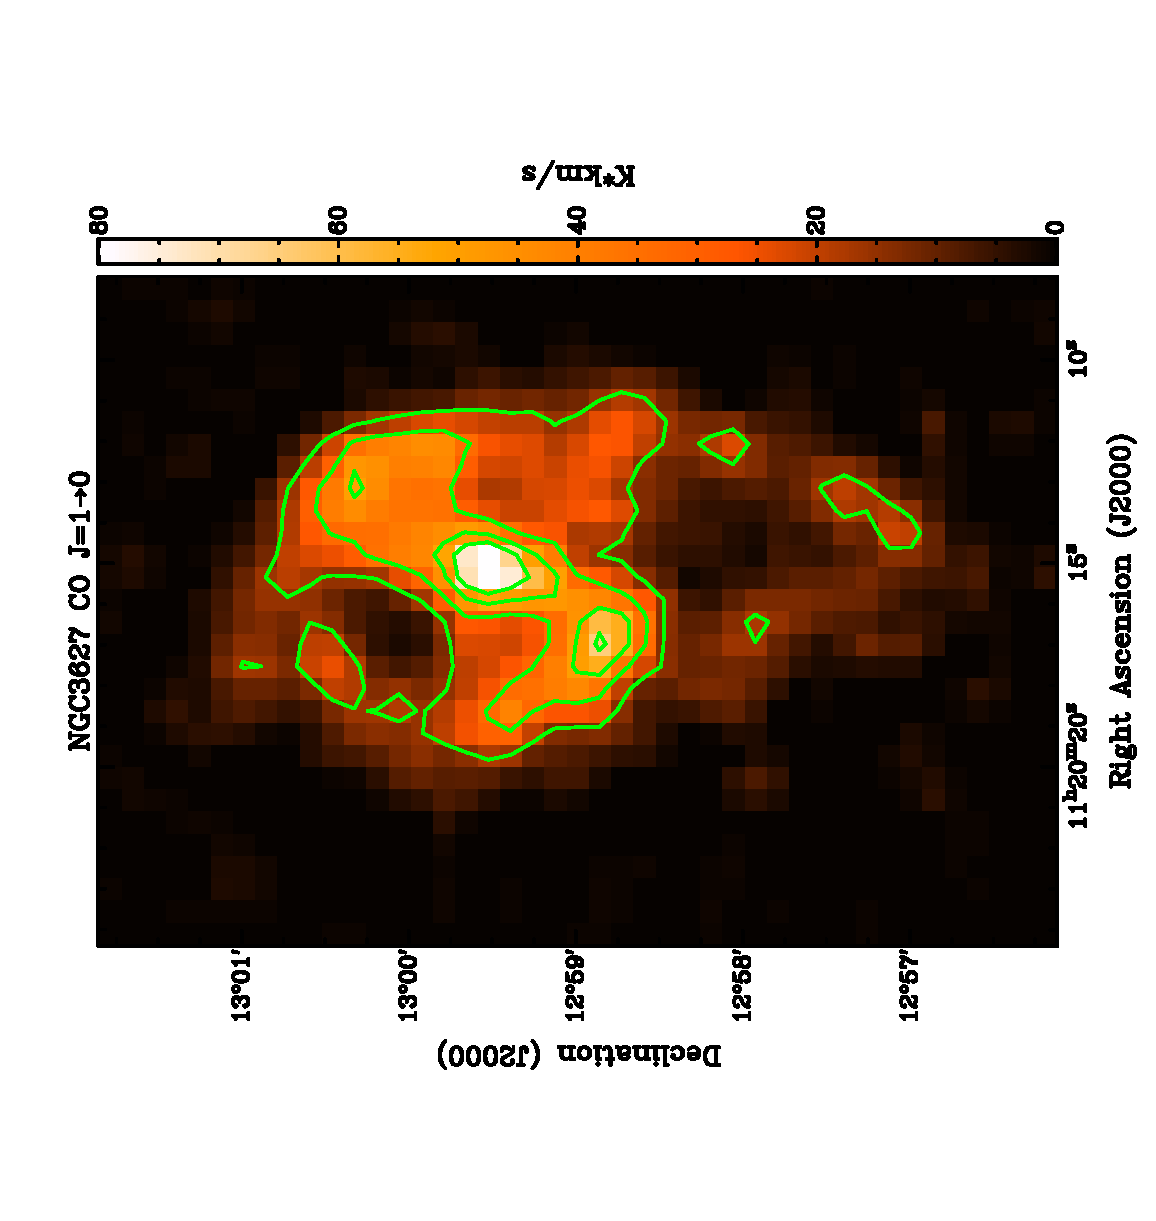
\includegraphics[width=1.\textwidth, angle=270]{obs_imgs/10_rem.eps}
  \caption[NGC3627 CO J=1-0 Observations]{Residual of the MAKEMAP filtering of CO J=1-0 observations with 20\%, 40\%, 60\%, and 80\% contours.}
  \label{fig_co10}
\end{figure}

\begin{deluxetable}{cccc}
  \tablecolumns{4}
  \tablewidth{0pt}
  \tablecaption{Properties of NGC3627 Nobeyama 45-m Observations\label{tab_obs_n45}}
  \tablehead{\colhead{Observation} & \colhead{Beam Properties } & \colhead{RMS} & \colhead{Percentage of Emission Removed} \\ 
  & $\theta_{beam}$ & \it{[K km/s]}}
  \startdata
    CO J=1-0 & 15.0$\arcsec$ & 0.681 & 20\% \\
  \enddata
\end{deluxetable}

\subsection{Hetrodyne Receiver Array CO-Line Extragalactic Survey (HERACLES)}

The CO J=2-1 line was used to determine a CO ${2-1} / {1-0}$ line ratio which can be used to trace a gradient in $\alpha_{CO}$ and hint towards regions of high star formation \citep{reuter1996}.  We used the CO J=1-0 data from the Nobeyama 45-m telescope ($\S$ \ref{nob_sec}), and CO J=2-1 from the Hetrodyne Reciever Array CO-Line Extragalactic Survey (HERACLES) using the IRAM 30-m telescope.  The main goal of HERACLES was to quantify the relationship between atomic and molecular gas and star formation using a large sample of galaxies \citep{leroy2009}.  The galaxies chosen were targets contained in THINGS that were within the observing limits of the IRAM 30-m telescope.  The final CO J=2-1 image can be seen in Figure \ref{fig_co21} and the image properties can be seen in Table \ref{tab_obs_heracles} with 8$\arcsec$ by 8$\arcsec$ pixels.

\begin{figure}
  \centering

  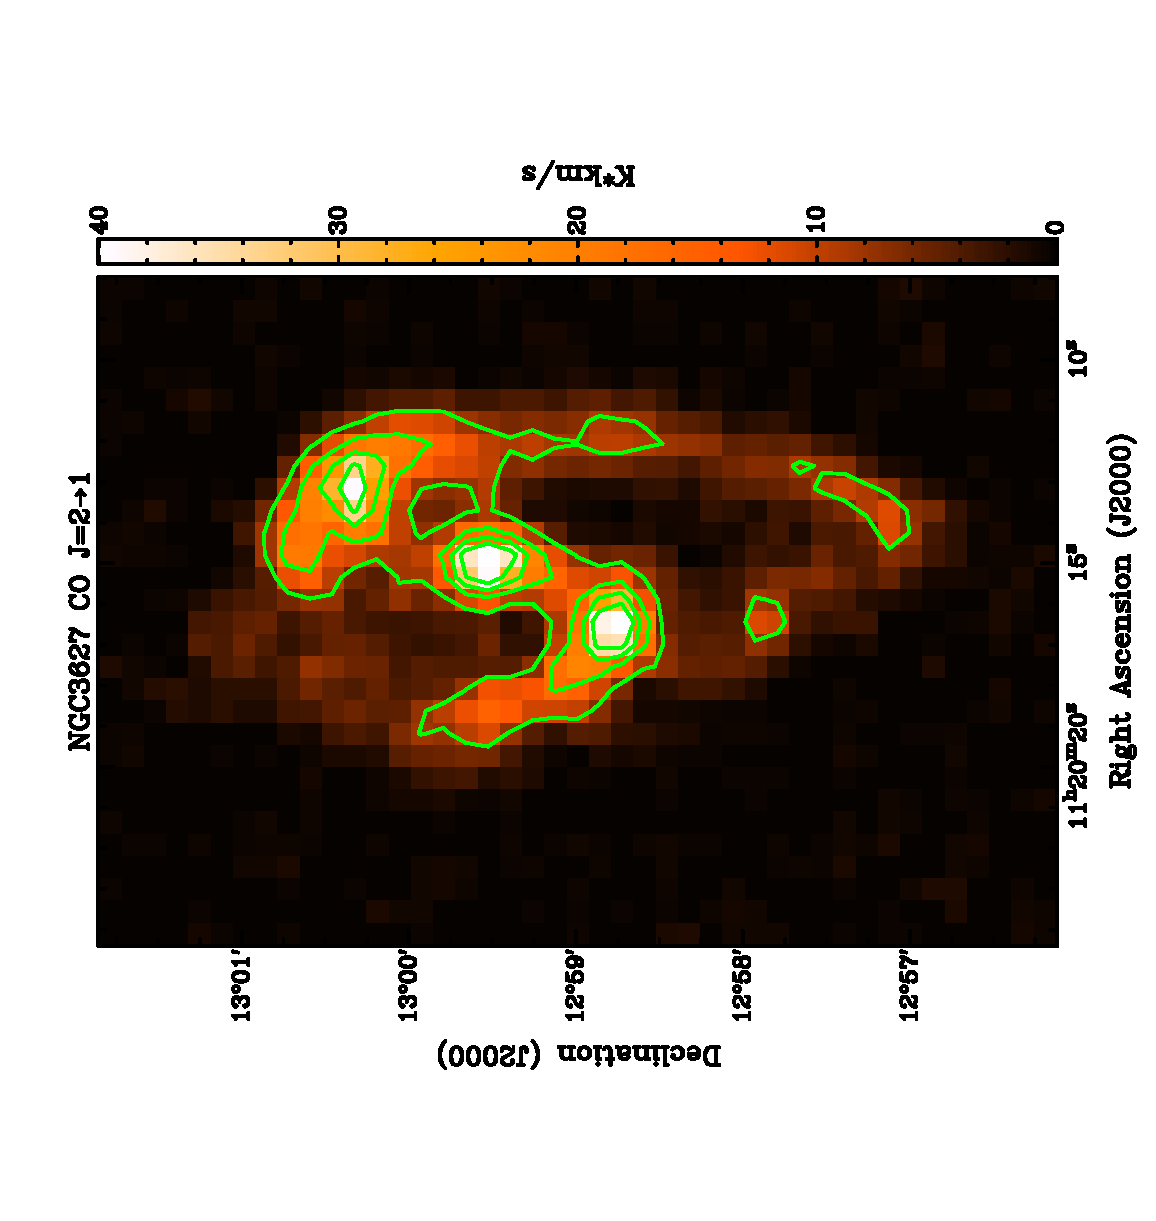
\includegraphics[width=1.\textwidth, angle=270]{obs_imgs/21_rem.eps}
  \caption[NGC3627 CO J=2-1 Observations]{Residual of the MAKEMAP filtering of CO J=2-1 observations with 20\%, 40\%, 60\%, and 80\% contours.}
  \label{fig_co21}
\end{figure}

\begin{deluxetable}{cccc}
  \tablecolumns{4}
  \tablewidth{0pt}
  \tablecaption{Properties of NGC3627 HERACLES Observations\label{tab_obs_heracles}}
  \tablehead{\colhead{Observation} & \colhead{Beam Properties } & \colhead{RMS} & \colhead{Percentage of Emission Removed} \\
  & $\theta_{beam}$ & \it{[K km/s]}}
  \startdata
    CO J=2-1 & 13.0$\arcsec$ & 0.305 & 7\% \\
  \enddata
\end{deluxetable}

\subsection{The HI Nearby Galaxy Survey (THINGS)}

To determine the gas-to-dust ratio we had to determine the total amount of gas present which includes both atomic and molecular hydrogen.  We approximated the amount of molecular hydrogen by using CO J=1-0, and measured the amount of atomic hydrogen (HI) present from The HI Nearby Galaxy Survey (THINGS) designed to observe HI emission in nearby galaxies with the extreme spatial resolution of the Very Large Array (VLA).  Targets in THINGS included many of the SINGS targets with the exception of known HI poor sources (E/S0 type galaxies), dynamically complex systems (edge-on spirals), and large extended galaxies found in the Local Group \citep{walter2008}.  The resolution and rms of the filtered image are shown in Table \ref{tab_obs_things} for 8$\arcsec$ by 8$\arcsec$ pixels.  The final data product is shown in Figure \ref{fig_HI} and has been converted to M$_\odot$ pc$^{-2}$ using 

\begin{equation}\label{eq:things_surf_den}
  M_{HI}\left[ M_\odot \right]=2.36 \times 10^5 D^2 \times \sum_{i}S_i\Delta v
\end{equation}

\noindent \citep{walter2008} and then dividing by the pixel area in pc$^2$ where D is the distance, and $\sum_{i}$S$_i\Delta$v is the first moment of the flux.  Since most of the HI emission is diffuse and extended, the filtering process removed nearly all of the HI features.  The removal of most of the HI resulted in a severe depression feature resempling a bowl in the middle of the map around the galaxy that was lower than the mean background value of the map.  The bowling effect ended up furthur lowering the surface densities of the final maps by lowering the peak value and removing a significant fraction of the surface density.

\begin{figure}
  \centering
  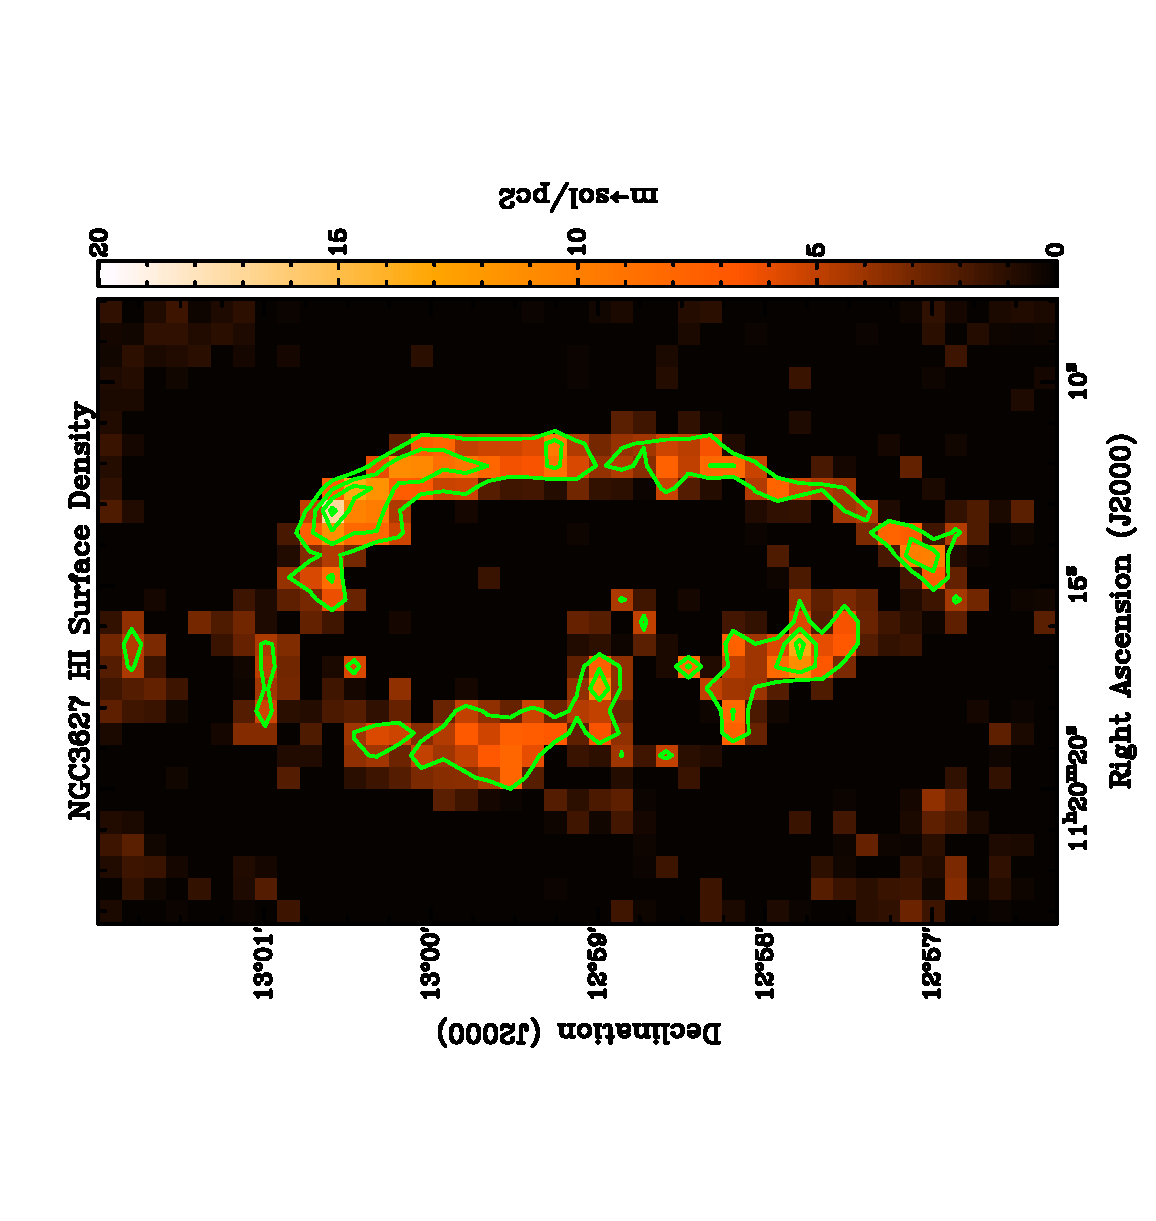
\includegraphics[width=1.\textwidth,angle=270]{obs_imgs/HI_rem.eps}
  \caption[NGC3627 HI Observations]{Residual of the MAKEMAP filtering of HI observations with 20\%, 40\%, 60\%, and 80\% contours.}
  \label{fig_HI}
\end{figure}

\begin{deluxetable}{cccccc}
  \tablecolumns{6}
  \tablewidth{0pt}
  \tablecaption{Properties of NGC3627 THINGS Observations\label{tab_obs_things}}
  \tablehead{\colhead{Observation} & \multicolumn{3}{c}{Beam Properties} & \colhead{RMS} & \colhead{Percentage of Surface Density Removed} \\
   & $\theta_{maj}$ & $\theta_{min}$ & $\theta_{PA}$ & \it{[$M_{\odot} / pc^2$]}}
  \startdata
    HI & 10.6$\arcsec$ & 8.85$\arcsec$ & -48.0$^\circ$ & 0.760 & $>$99\% \\  
  \enddata
\end{deluxetable}

\section{Data Preparation for Analysis}\label{data_agree}

Looking at Figures \ref{fig_450}, \ref{fig_850} and comparing them with the ancillary data images in Figures \ref{fig_100}-\ref{fig_HI} it is clear the data do not agree completely even with their extended sructure removed.  Other than the presence of the large scale/extended structure prior to filtering, the main difference between each image is its resolution, in particular the beam shape of the 450$\mu$m data.  We have taken several steps to correct for these disagreements and maximize the compatibility of the data.  In order to account for the varying beam resolutions, we use a gaussian convolution to degrade the resolution of our maps to the largest beam size in our dataset, $\sigma_{max}$=36$\arcsec$.  An appropriate convolution beam width is determined by 

\begin{equation}\label{eq:gaus_kern}
  \sigma_{desire} = \sqrt{\sigma_{max}^2 - \sigma_{given}^2}
\end{equation}

\noindent where $\sigma_{desire}$ is the desired beam width, $\sigma_{max}$ is the beam size we are convolving to, and $\sigma_{given}$ is the beam size we are convolving from.  However, equation \ref{eq:gaus_kern} only works when the beams are well approximated by a single gaussian which is not the case for the 450$\mu$m beam.  The steps taken to match the resolution of the 450$\mu$m beam with the rest of the data set are given in $\S$\ref{450_fix_sec}.  

Removing any large scale structure from our ancillary data is implemented using a feature built into MAKEMAP that allows us to add fake sources into the data during production.  The fake source implementation allows us to remove the same amount of large scale structure from our ancillary data as was removed from the SCUBA-2 data.  The steps taken to prepare the ancillary data are described in $\S$\ref{fakesource_sec}.

%The largest difference in Ability of Herschell to observe submm unimpeded by atmo and the configuration setup of THIGNs allows for a bit of extended structure to arise in NGC3627.

\subsection{Accounting for the 450$\mu$m Error Beam}\label{450_fix_sec}

Taking the 450$\mu$m error beam into consideration is different from a normal beam convolution in the sense that we are not convolving the higher resolution map to the lowest resolution.  Instead we are adding in an error beam similar to the error beam found in the 450$\mu$m observations.  We have to take these steps because convolving a double gaussian beam with a single gaussian kernel will not sufficiently remove the error component of our beam resulting in a poor approximation to the wings of our beam shape.

In order to accommodate the 450$\mu$m map's error beam, we used a method employed by another SCUBA-2 legacy survey, the Gould Belt Survey.  This method uses the distributive nature of the Fourier transform to create similar error components in the beams we were convolving to and from.  Carrying out this convolution involves breaking the 450$\mu$m beam into its two components, $X_{\alpha}$ and $X_{\beta}$, to represent the main beam and error beam.  The values of the main beam amplitude, $X_\alpha$, and error beam amplitude, $X_\beta$, will sum to one so the height of the total beam is normalized to one.  The poorest resolution beam, $X_{max}$, is convolved with the two components $X_\alpha$ and $X_\beta$ and the resulting beams are added together.  This process produces an equivalent two component beam to the 450$\mu$m beam convolved with $X_{max}$.  The relationship can be expressed as 

\begin{equation} \label{eq_GBSmethod}
  \begin{split}
    X_{max} \ast X_{\alpha} + X_{max} \ast X_{\beta} & = \left(X_{\alpha} + X_{\beta}\right) \ast X_{max} \\
     & = X_{450\mu m} \ast X_{max}
   \end{split}
\end{equation}

\noindent where $X_{max}$ is the poorest resolution beam, $X_{\alpha}$ and $X_{\beta}$ are the main and error beam of the 450$\mu$m observations, and $X_{450\mu m}$ is the double gaussian beam shape of the 450$\mu$m observations.

\subsection{Extended Structure Removal via MAKEMAP}\label{fakesource_sec}

%adjusting the beam sizes to make the 450 beam work

%from the ancillary data set -- describes the fakesource stuff
Due to the combination of methods used in MAKEMAP, large scale/extended structure is removed from the final SCUBA-2 images.  However, in all of our ancillary data the large scale emission was present in the initial maps.  The removal of the extended features from our ancillary data was carried out by passing the data through MAKEMAP using a special function called fakemap.  Using fakemap allows us to pass an image though the SCUBA-2 processing and have it added into the image being processed.  We use the 850$\mu$m map as our base image for the filtering process and add the ancillary data to the 850$\mu$m image.  The output image then consists of the sum of the ancillary data and the 850$\mu$m map.  Finally, the ancillary data were isolated by subtracting the 850$\mu$m image from the fakemap output image.  

Preparing the data to be added via fakemap consists of either converting the images from their native units into pW using the 850$\mu$m flux calibration factor and scaling down to match the observed signal or by just applying a scaling factor.  Which method is used is based on the desired units of the final map, and can be separated by what purpose the data had in our analysis.

The data used in the SED fitting (KINGFISH and NGLS) were scaled to pW so they could have a similar reduction and calibration process as the SCUBA-2 maps.   The KINGFISH data are regridded to a 2$\arcsec$ by 2$\arcsec$ pixel size and have the appropriate calibration factor from \cite{dempsey2013} applied to convert from either MJy/sr to pW in the case of the 250$\mu$m, 350$\mu$m, and 500$\mu$m or from Jy/pixel to pW for the 100$\mu$m and 160$\mu$m.  Converting the CO J=3-2 data requires the final product to be in the same units as the 850$\mu$m observations in order to properly remove the molecular gas contribution.  Converting from K km/s to mJy/beam involves applying a scaling constant of 0.70 [mJy/beam][K km/s]$^{-1}$ \citep{drabek2012} prior to applying the 850$\mu$m flux calibration factor to convert to pW.  

After the data has been converted to pW, the image used in fakemap is then scaled down to the same order of magnitude as the base image using a scaling factor specified prior to the map production.  After the fakemap image has been processed and the 850$\mu$m map subtracted, the maps are scaled back up using the same scaling factor used to scale them down and calibrated using the same flux calibration factors as the 850$\mu$m map and scaled to an 8$\arcsec$ by 8$\arcsec$ grid.  The amount of extended flux lost from the KINGFISH and NGLS images is shown in Tables \ref{tab_obs_kfish} and \ref{tab_obs_NGLS}.  This process is illustrated in Figure \ref{fig_100_transform} from the original Herschel 100$\mu$m map, to the final image used in SED fitting convolved to the 500$\mu$m beam resolution, 36.0$\arcsec$.

\begin{figure}
  \centering
  \begin{subfigure}[t]{.48\textwidth}
    \centering
    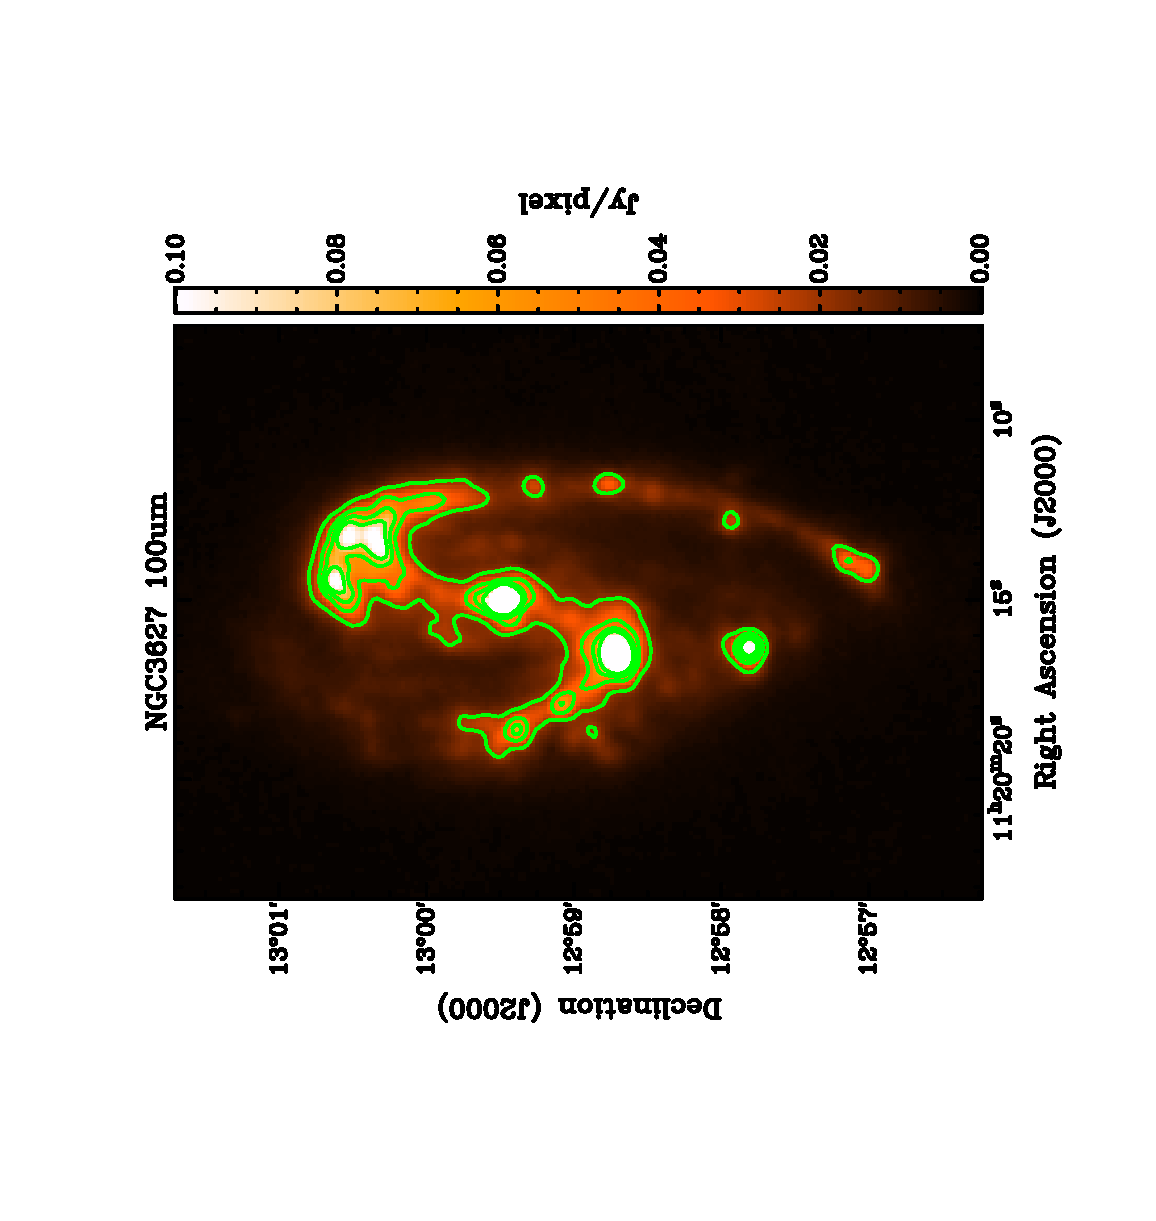
\includegraphics[width=1.\linewidth, angle=270]{obs_imgs/100_orig.eps}
    \caption{Herschel 100$\mu$m image of NGC3627 with 1.7$\arcsec$ by 1.7$\arcsec$ pixels.}
  \end{subfigure}%
  \quad
  \begin{subfigure}[t]{.48\textwidth}
    \centering
    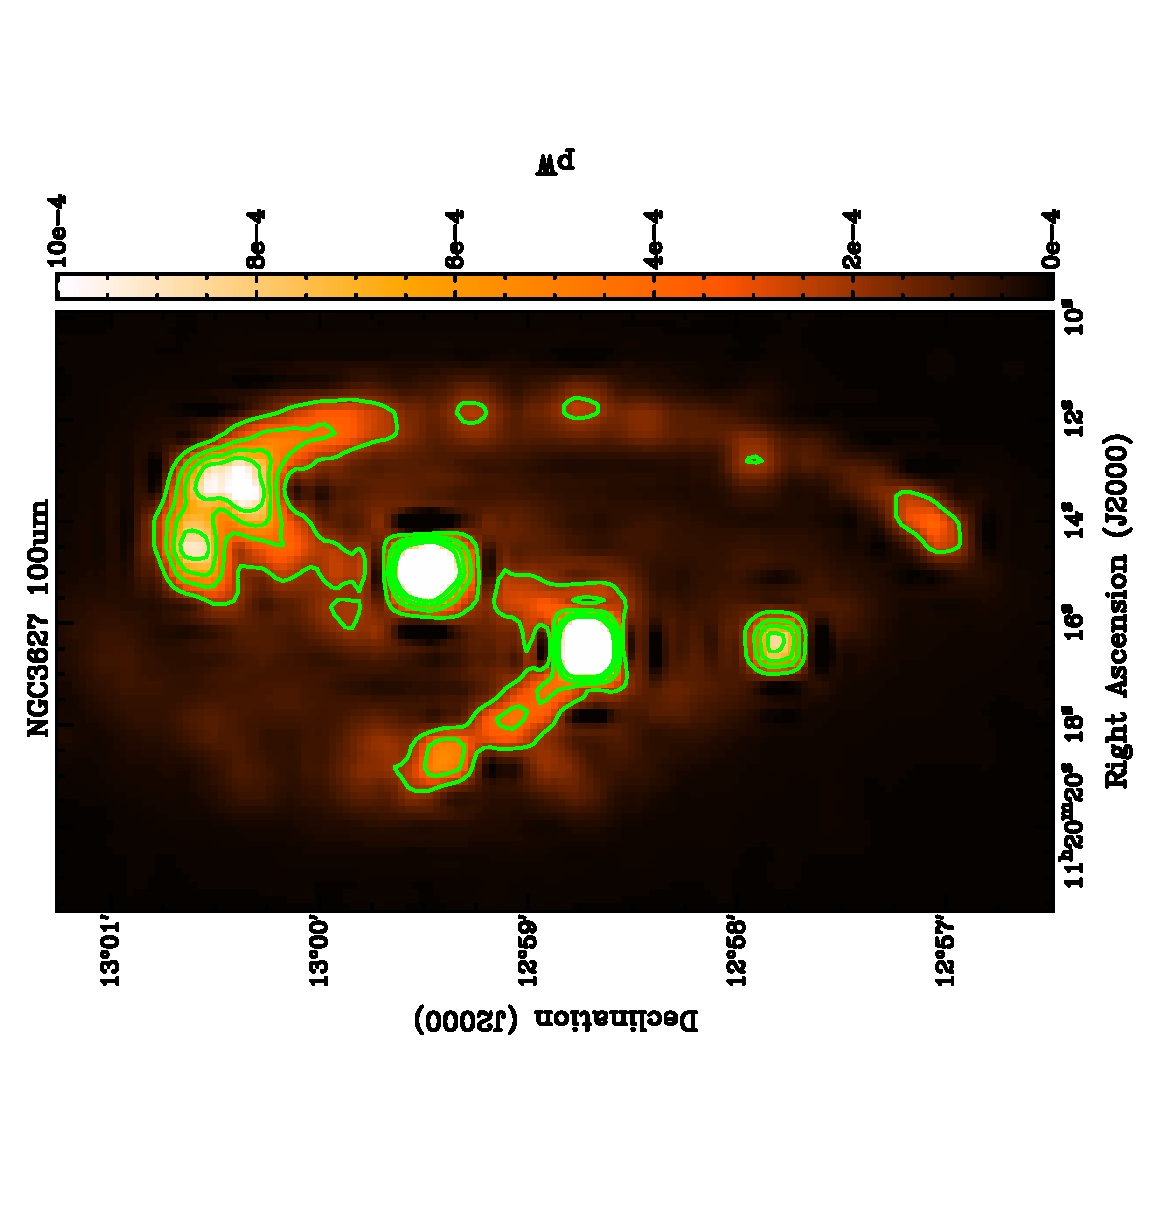
\includegraphics[width=1.\linewidth, angle=270]{obs_imgs/100_align.eps}
    \caption{Herschel 100$\mu$m image converted to pW and rescaled to a 2$\arcsec$ by 2$\arcsec$ pixel grid.}
  \end{subfigure}%

  \begin{subfigure}[t]{.45\textwidth}
    \centering
    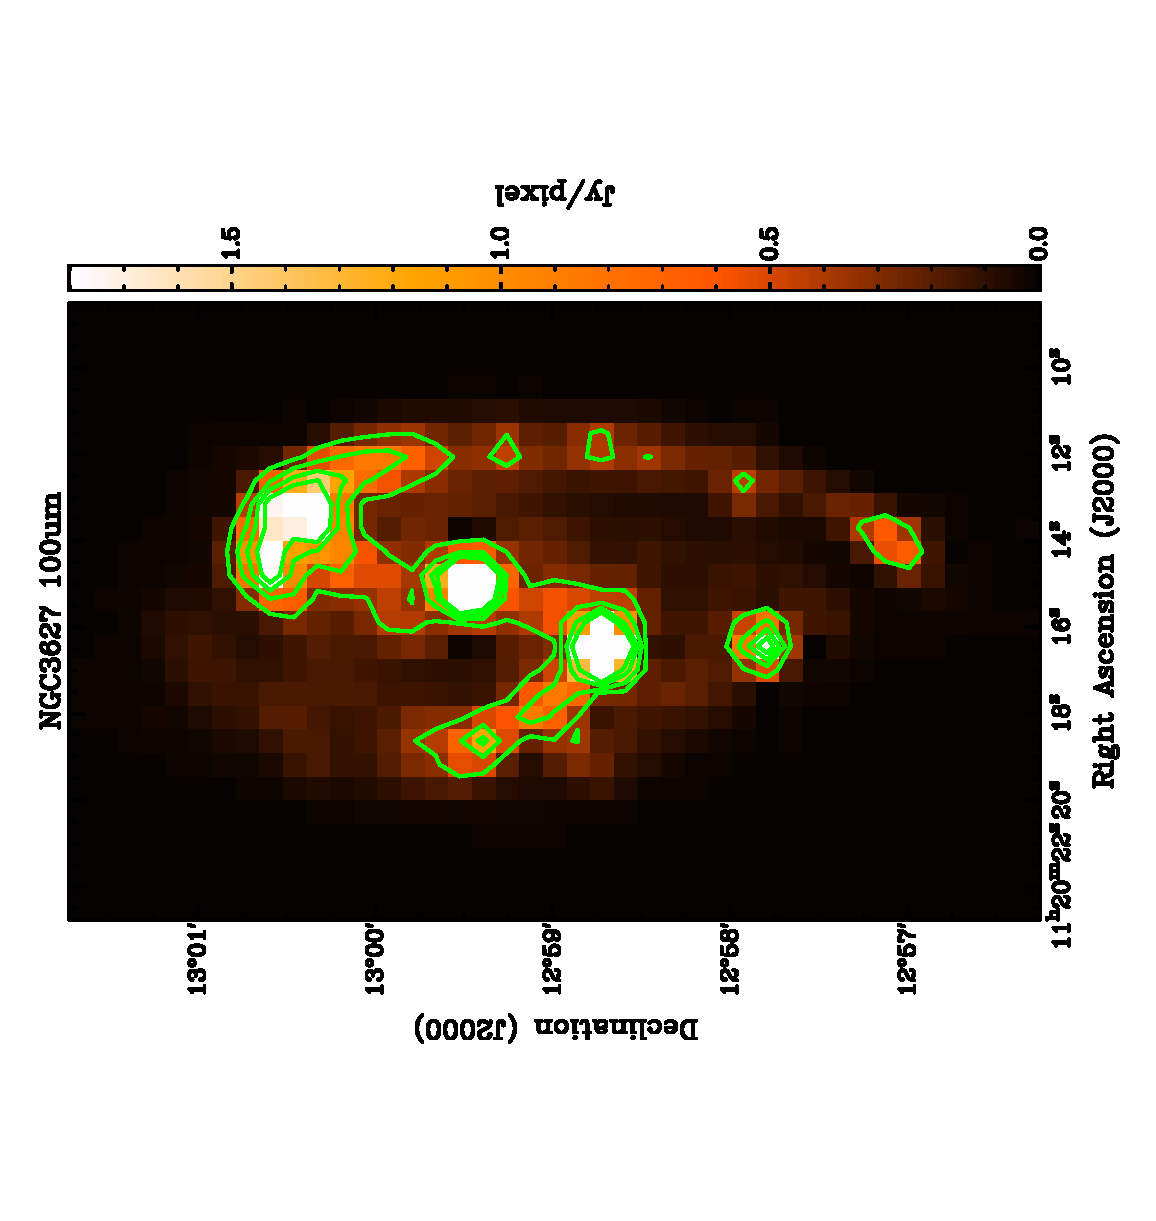
\includegraphics[width=1.\textwidth,angle=270]{obs_imgs/100_rem.eps}
    \caption{100$\mu$m map of NGC3627 after large scale structure has been removed and rescaled to an 8$\arcsec$ by 8$\arcsec$ grid.}
  \end{subfigure}%
  \quad
  \begin{subfigure}[t]{0.45\textwidth}
    \centering
    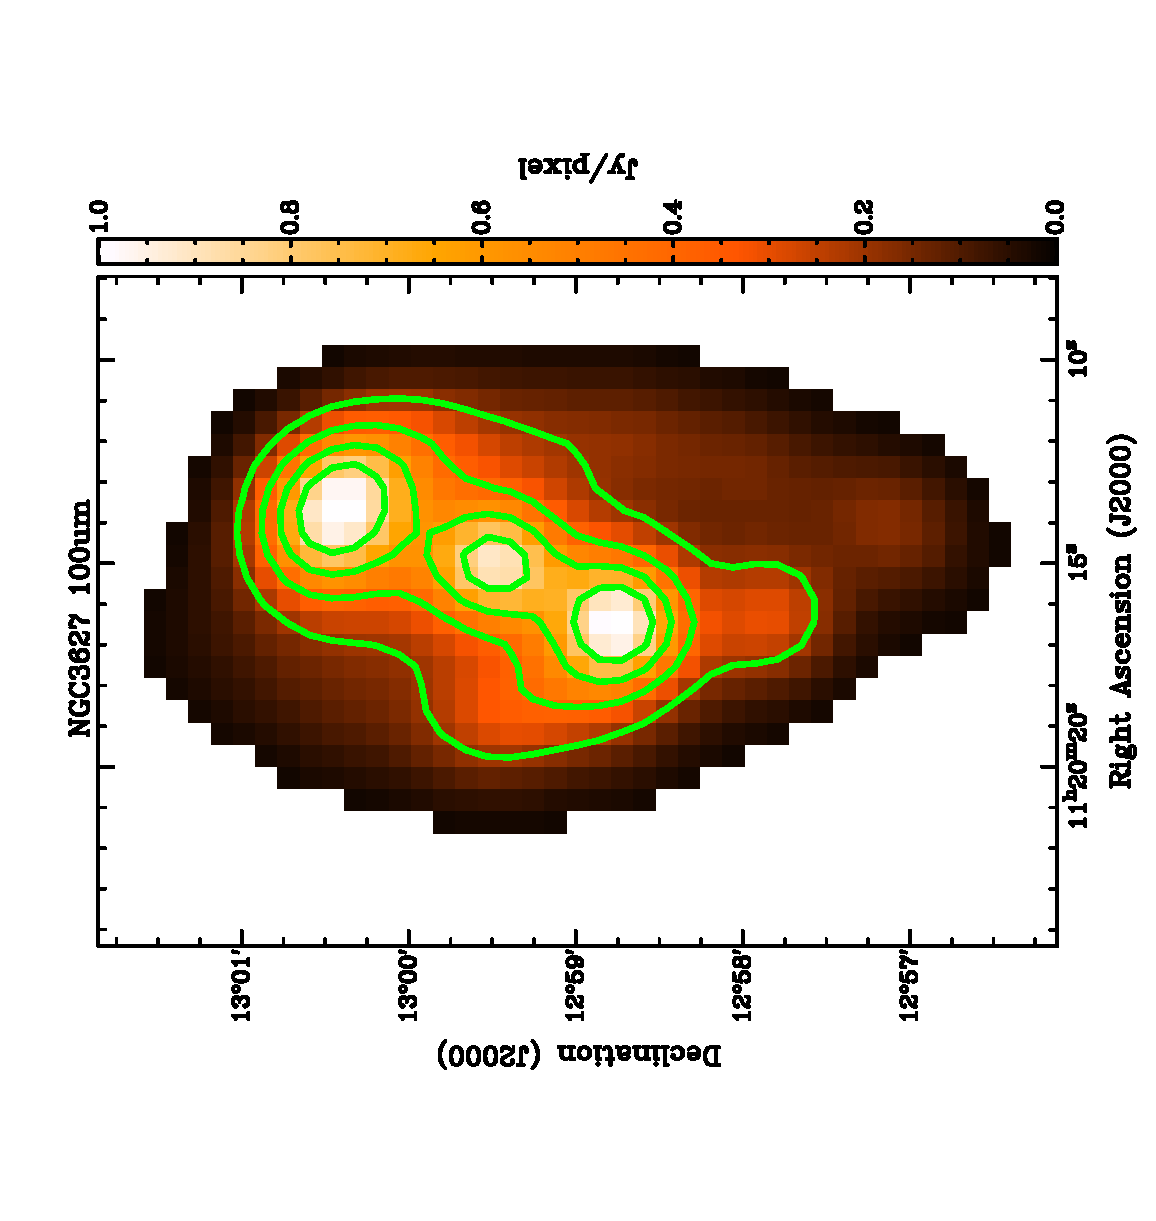
\includegraphics[width=1.\textwidth,angle=270]{obs_imgs/100_sed_use.eps}
    \caption[100$\mu$m Filtering Steps]{100$\mu$m map with extended structure removed and convolved to final resolution of 36.0$\arcsec$ with a 5$\sigma$ cut applied.}
  \end{subfigure}
  \caption[100$\mu$m Filtering Steps]{The 100$\mu$m image from the beginning of processing to the end of processing.  All of the contours shown are 20\%, 40\%, 60\%, and 80\%.}
  \label{fig_100_transform}
\end{figure}
  

The rest of the ancillary data are used in calculating a dust to gas ratio, and follow nearly the same process as the SED data filtering.  The major difference is the CO J=1-0, CO J=2-1 and HI maps need to remain in their original units of K km/s and M$_\odot$/pc$^2$.  This requirement simplified the process by only requiring a scaling factor of 0.001 to be applied to the original maps.  After the image is scaled, it is filtered using the fakesource option in MAKEMAP with the 850$\mu$m observation as the base image.  The atomic and molecular gas maps were then isolated in the same fashion as the KINGFISH and NGLS by subtracting the 850$\mu$m map.  Then they were rescaled back to their original values, fit to an 8$\arcsec$ by 8$\arcsec$ grid and finally convolved to a 36.0$\arcsec$ resolution.  The process is illustrated in Figure \ref{fig_HI_transform}.  The amount of emission lost is shown in tables \ref{tab_obs_n45}, \ref{tab_obs_heracles}, and \ref{tab_obs_things}.

\begin{figure}
  \centering
  \begin{subfigure}[t]{.48\textwidth}
    \centering
    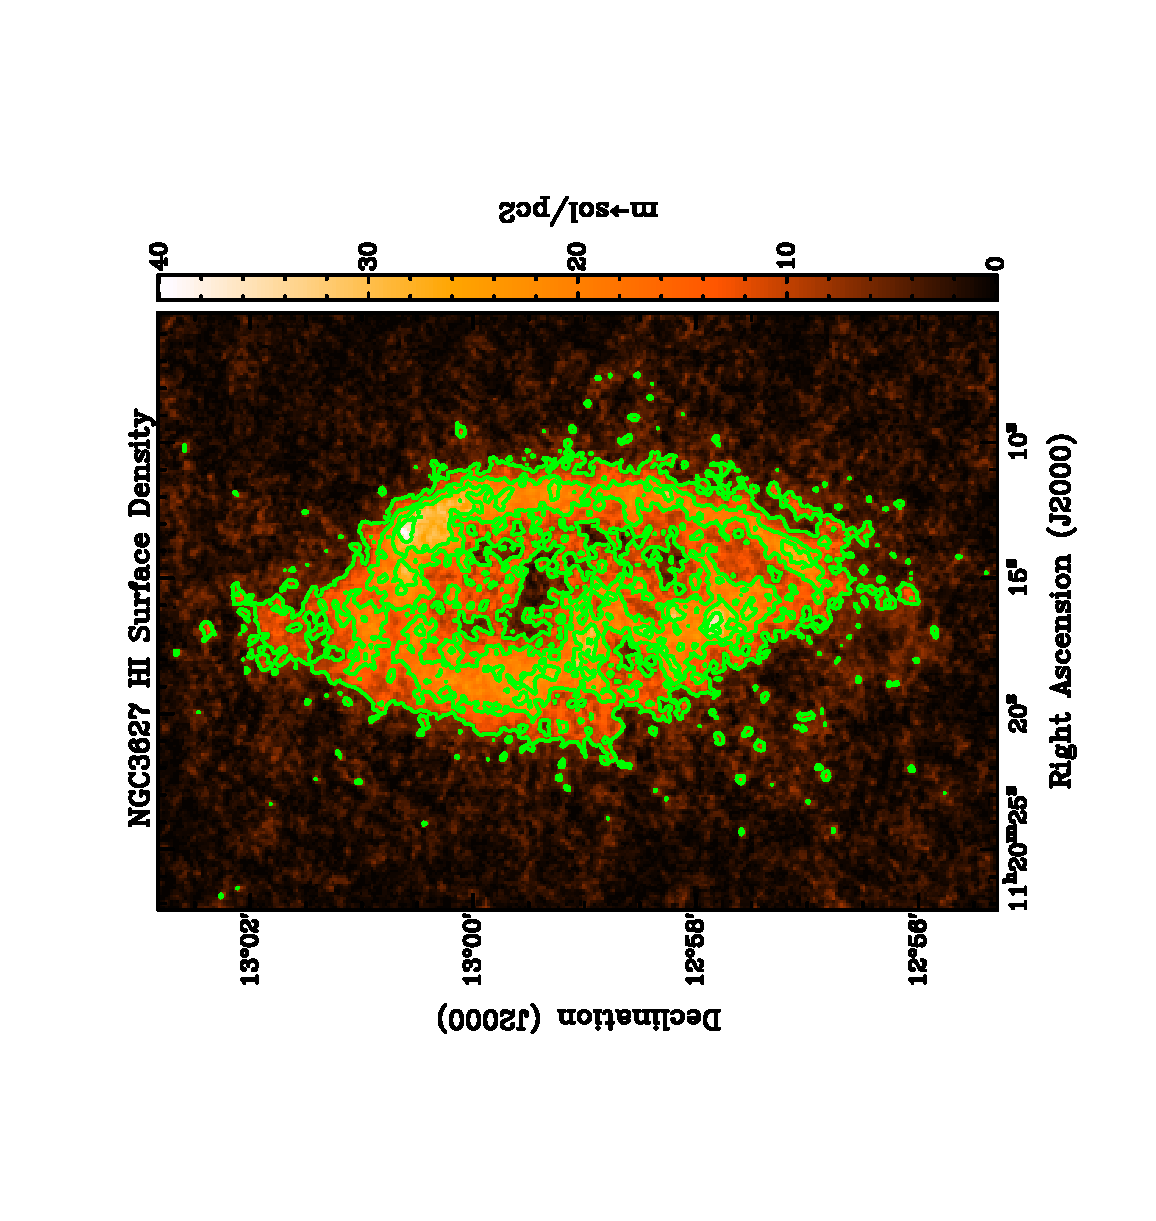
\includegraphics[width=1.\linewidth, angle=270]{obs_imgs/HI_orig.eps}
    \caption{HI surface density map of NGC3627 with 1.5$\arcsec$ by 1.5$\arcsec$ pixels.}
  \end{subfigure}%
  \quad
  \begin{subfigure}[t]{.48\textwidth}
    \centering
    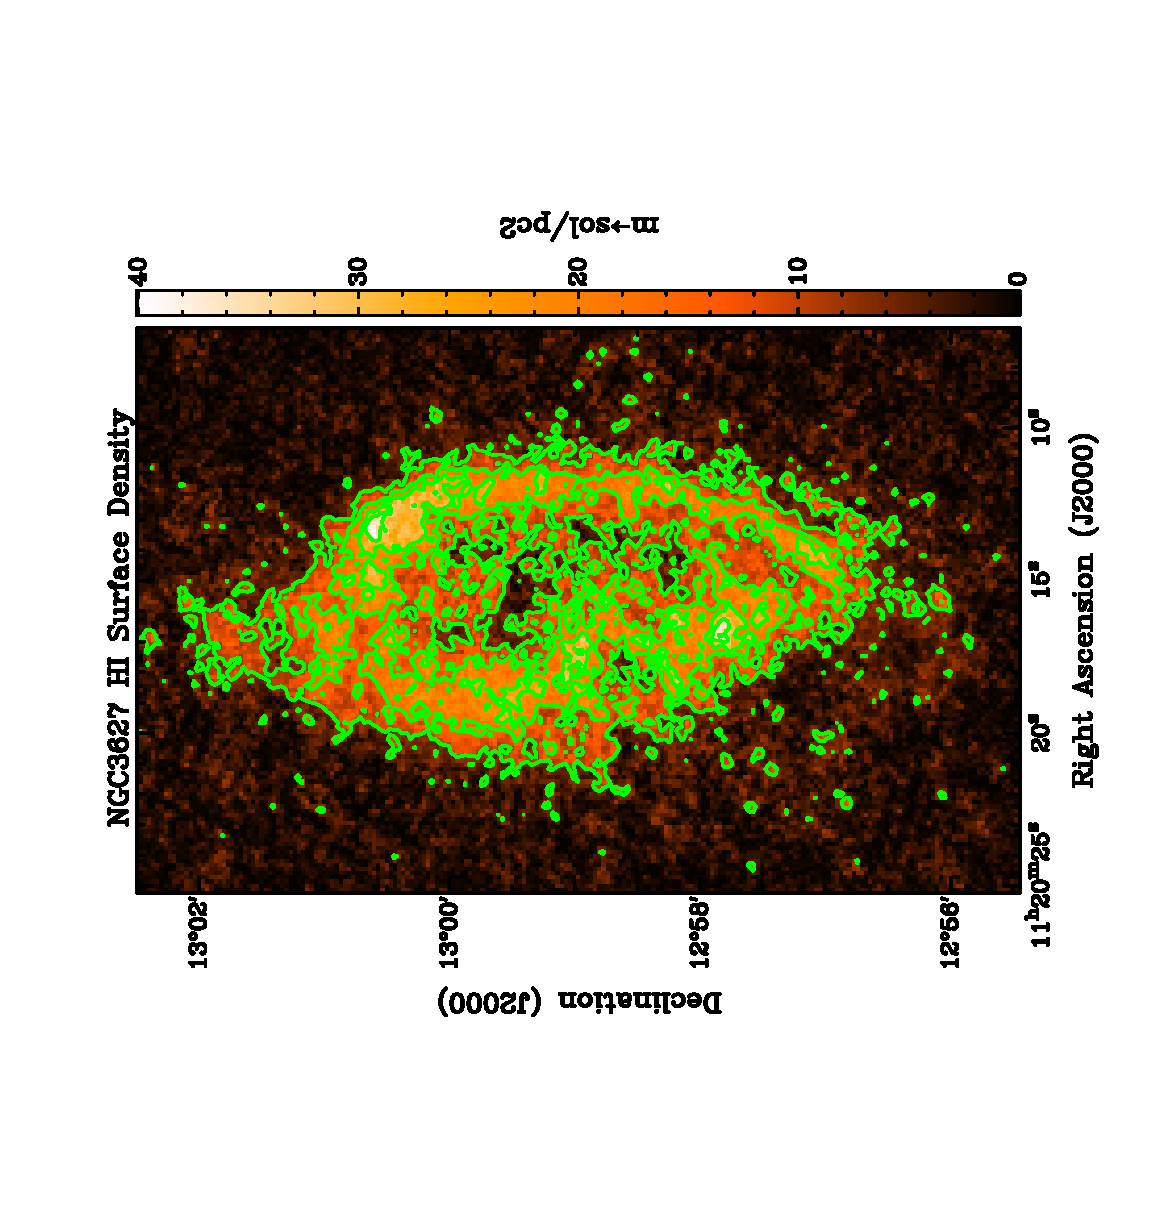
\includegraphics[width=1.\linewidth, angle=270]{obs_imgs/HI_align.eps}
    \caption{HI surface density map rescaled to a 2$\arcsec$ by 2$\arcsec$ pixel grid.}
  \end{subfigure}%

  \begin{subfigure}[t]{.45\textwidth}
    \centering
    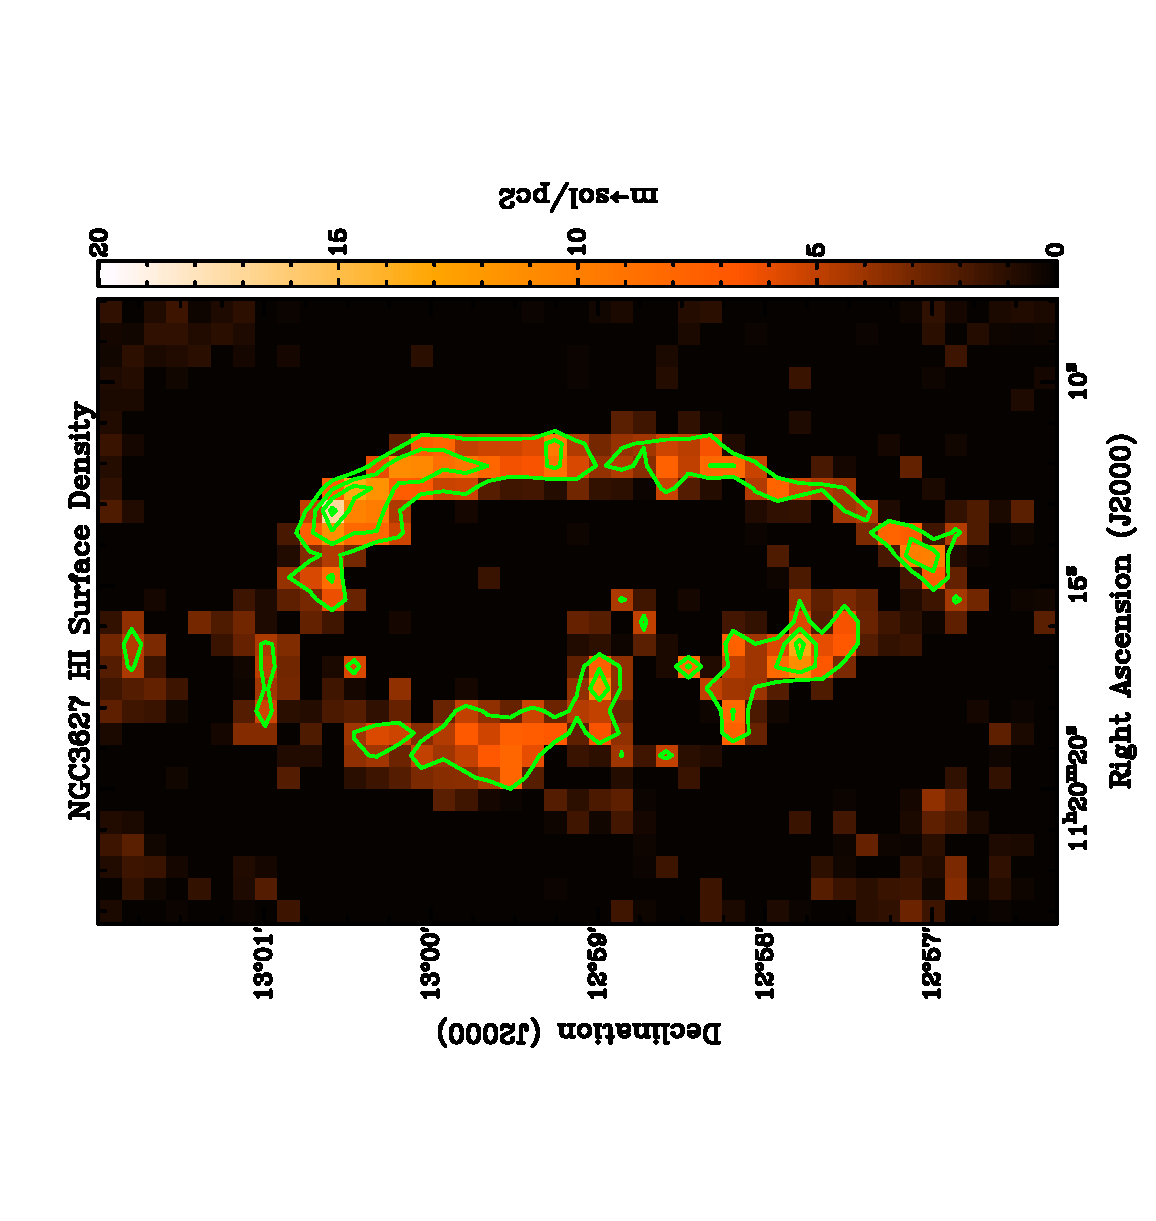
\includegraphics[width=1.\textwidth,angle=270]{obs_imgs/HI_rem.eps}
    \caption{HI surface density map of NGC3627 after large scale structure has been removed and rescaled to an 8$\arcsec$ by 8$\arcsec$ grid.}
  \end{subfigure}%
  \quad
  \begin{subfigure}[t]{0.45\textwidth}
    \centering
    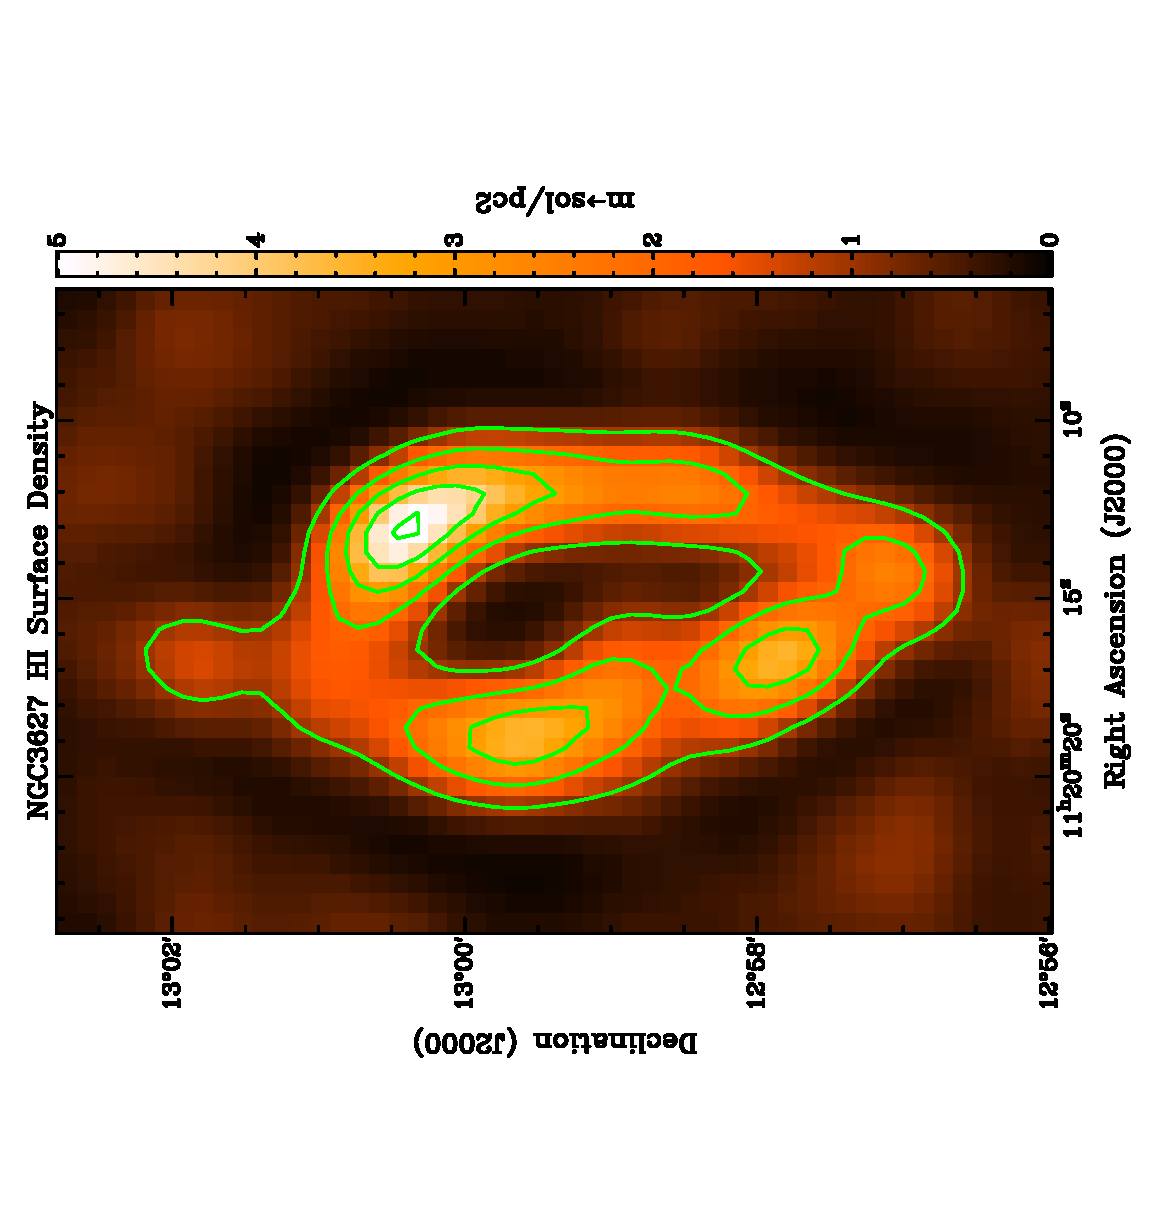
\includegraphics[width=1.\textwidth,angle=270]{obs_imgs/HI_use.eps}
    \caption[100$\mu$m Filtering Steps]{HI surface density map with extended structure removed and convolved to final resolution of 36.0$\arcsec$.}
  \end{subfigure}
  \caption[HI surface density filtering Steps]{The HI surface density maps from the beginning of processing to the end of processing.  The contours in the top row are 30\%, 60\% and 90\%, and the contours in the bottom row are 20\%, 40\%, 60\%, and 80\%.}
  \label{fig_HI_transform}
\end{figure}
 
